\RequirePackage[l2tabu,orthodox]{nag}
% TODO: decide if one-sided/two-sided
%\documentclass[headsepline,footsepline,footinclude=false,fontsize=11pt,paper=a4,listof=totoc,bibliography=totoc,BCOR=12mm,DIV=12]{scrbook} % two-sided
\documentclass[headsepline,footsepline,footinclude=false,oneside,fontsize=11pt,paper=a4,listof=totoc,bibliography=totoc]{scrbook} % one-sided

\PassOptionsToPackage{table,svgnames,dvipsnames}{xcolor}

\usepackage[utf8]{inputenc}
\usepackage[T1]{fontenc}
\usepackage[sc]{mathpazo}
\usepackage[american]{babel}
\usepackage[autostyle]{csquotes}
\usepackage[%
  backend=biber,
  url=false,
  style=alphabetic,
  maxnames=4,
  minnames=3,
  maxbibnames=99,
  firstinits,
  uniquename=init]{biblatex} % TODO: adapt bibliography style
\usepackage{graphicx}
\usepackage{scrhack} % necessary for listings package
\usepackage{listings}
\usepackage{lstautogobble}
\usepackage{tikz}
\usepackage{pgfplots}
\usepackage{pgfplotstable}
\usepackage{booktabs}
\usepackage[final]{microtype}
\usepackage{caption}
\usepackage[hidelinks]{hyperref} % hidelinks removes colored boxes around references and links
\usepackage[toc,nonumberlist,acronym]{glossaries} % TODO: remove if glossary not needed
\usepackage[export]{adjustbox} %positioning of figures and tables
\usepackage{subcaption}
\usepackage{multirow}


%\bibliography{bibliography/literature}

\setkomafont{disposition}{\normalfont\bfseries} % use serif font for headings
\linespread{1.5} % adjust line spread for mathpazo font

% Settings for glossaries TODO: remove the following block if glossary not needed
%\renewcommand{\glsnamefont}[1]{\normalfont\bfseries #1} % use serif font for
% glossary entry titles
%\makeglossaries{}

% Settings for pgfplots
\pgfplotsset{compat=newest} % TODO: adjust to your installed version
\pgfplotsset{
  % For available color names, see http://www.latextemplates.com/svgnames-colors
  cycle list={CornflowerBlue\\Dandelion\\ForestGreen\\BrickRed\\},
}

% Settings for lstlistings
\lstset{%
  basicstyle=\ttfamily,
  columns=fullflexible,
  autogobble,
  keywordstyle=\bfseries\color{MediumBlue},
  stringstyle=\color{DarkGreen}
}

% Basic information for cover & title page
\newcommand*{\getUniversity}{Der Technischen Universität München}
\newcommand*{\getFaculty}{Fakultät für Informatik}
\newcommand*{\getTitle}{Scenarios for Distributed User Interfaces for Single-User Recommender Systems}
\newcommand*{\getTitleGer}{Szenarien für verteilte Benutzerschnittstellen für Empfehlungssysteme für einzelne Benutzer}
\newcommand*{\getAuthor}{Wessam Gharib Abdrabo}
\newcommand*{\getDoctype}{Master's Thesis in Informatics}
\newcommand*{\getSupervisor}{Prof. Dr. Johann Schlichter}
\newcommand*{\getAdvisor}{Dr. rer. nat. Wolfgang W\"{o}rndl}
\newcommand*{\getSubmissionDate}{November 16, 2015}
\newcommand*{\getSubmissionLocation}{Munich}

% TODO: add custom commands etc.


% TODO: remove if glossary not needed
\newglossaryentry{computer}
{
  name=computer,
  description={is a machine that\ldots}
}

\newacronym{tum}{TUM}{Technische Universität München}


\begin{document}

\begin{titlepage}
  % HACK for two-sided documents: ignore binding correction for cover page.
  % Adapted from Markus Kohm's KOMA-Script titlepage=firstiscover handling.
  % See http://mirrors.ctan.org/macros/latex/contrib/koma-script/scrkernel-title.dtx,
  % \maketitle macro.
  \oddsidemargin=\evensidemargin\relax
  \textwidth=\dimexpr\paperwidth-2\evensidemargin-2in\relax
  \hsize=\textwidth\relax

  \centering

  \vspace{40mm}
  \includegraphics[width=40mm]{logos/tum}

  \vspace{5mm}
  {\huge\MakeUppercase{\getFaculty{}}}\\

  \vspace{5mm}
  {\large\MakeUppercase{\getUniversity{}}}\\

  \vspace{20mm}
  {\Large \getDoctype{}}

  \vspace{15mm}
  {\huge\bfseries \getTitle{}}

  \vspace{15mm}
  {\LARGE \getAuthor{}}

  \vspace{20mm}
  \includegraphics[width=20mm]{logos/faculty}
\end{titlepage}


\frontmatter{}

\begin{titlepage}
  \centering

  \vspace{40mm}
  \includegraphics[width=40mm]{logos/tum}

  \vspace{5mm}
  {\huge\MakeUppercase{\getFaculty{}}}\\

  \vspace{5mm}
  {\large\MakeUppercase{\getUniversity{}}}\\

  \vspace{20mm}
  {\Large \getDoctype{}}

  \vspace{10mm}
  {\huge\bfseries \getTitle{}}

  \vspace{5mm}
  {\huge\bfseries \getTitleGer{}}

  \vspace{10mm}
  \begin{tabular}{l l}
    Author: & \getAuthor{} \\
    Supervisor: & \getSupervisor{} \\
    Advisor: & \getAdvisor{} \\
    Submission Date: & \getSubmissionDate{} \\
  \end{tabular}

  \vspace{2mm}
  \includegraphics[width=20mm]{logos/faculty}
\end{titlepage}

\thispagestyle{empty}
\vspace*{0.8\textheight}
\noindent
I confirm that this \MakeLowercase{\getDoctype{}} is my own work and I have documented all sources and material used.

\vspace{15mm}
\noindent
\getSubmissionLocation{}, \getSubmissionDate{} \hspace{5cm} %\getAuthor{}

\cleardoublepage{}

\addcontentsline{toc}{chapter}{Acknowledgments}
\thispagestyle{empty}

\vspace*{2cm}

\begin{center}
{\usekomafont{section} Acknowledgments}
\end{center}

\vspace{1cm}
This work was made possible through the guidance and support of Dr. Wolfgang
W\"{o}rndl. I would like to thank TUM's chair of Applied Informatics - Cooperative
Systems, headed by Prof. Dr. Johann Schlichter, for the opportunity to work on
this thesis.\\
My deepest gratitude goes out to my parents, sister, and brothers for their
ceaseless support and much more.\\
I owe my thanks to my friends for contributing their time in participating
in the user study and in editing: Safey AbdelHalim, Sherif Abdellatif, Sara
Ezz ElArab, Nada ElNewehy, Ahmed ElShirbiny, Ahmed Gharib, Ibrahim Gharib, Shady
Hussein, Youmna Hussein, Ahmed Mesbah, Maha Shawky, and Daniel Von Bechen.\\
And lastly, thanks to the generosity of all the volunteering
user study participants for their time and effort.

\cleardoublepage{}

\chapter{\abstractname}
Distributed User Interfaces (DUIs) are user
interfaces which are distributed in time and space, among multiple platforms, displays, and
users. The emerging field of DUIs is one which has drawn the attention of
researchers in recent years, and which is found valuable to the field of ubiquitous and
interactive systems by an increasing number of studies. Notwithstanding the
evident value of DUIs, studies investigating the impact of using DUIs in
single-user recommendation systems are found lacking. Consequently, this work
bridges a gap in the research by providing a study of the impact of the application of DUIs on the experience of the users of
recommendation systems. In pursuit of our investigation, we developed two
prototype video recommendation mobile applications; Monolithic Interface
Recommender (MiRec), and Distributed Interface Recommender (DiRec). Sharing
mostly the same interface, DiRec additionally offers
the possibility of migrating parts of the UI between the mobile application and
a larger display (LD).
A user study was conducted in which participants used and evaluated both MiRec
and DiRec. Our study's results
show a significant difference between DiRec and MiRec in attractiveness (general
impression and likability), stimulation, and novelty measures, which posits the
existence of a strong interest in DUI recommender systems. Nonetheless, MiRec
was found more easy-to-learn and easier to understand than DiRec
which gives room for further investigation to pinpoint the reasons of DiRec's
relatively lower perspicuity measures.


\microtypesetup{protrusion=false}
\tableofcontents{}
\microtypesetup{protrusion=true}

\mainmatter{}

\chapter{Introduction}\label{chapter:introduction}

\section{Recommender Systems: Ubiquity and Distribution}
The explosive dimension of digital content has raised the need for tools that
could aid users in making informed decisions on consuming such content.
Recommendation systems are such tools that have become an integrated part of
everyday interaction with any digital content provider (such as Netflix, YouTube
Spotify), online store (such as Amazon), or even Google search engine. During
the past decade, it has become less and less uncommon for a user to get content
tailored to her taste based on recommendation algorithms that are ever-evolving,
providing sophisticated methods of implicitly building user profiles
through eliciting the user's preferences, or by mining users' search histories
or ratings for products and content. Recommendation algorithms varying from
content-based which is done based on item-to-item similarity, to context-based
which includes contextual information such as location and time in
recommendation, to collaborative filtering which takes into account similar
users' profiles, all provide a number of solutions to recommendation
applications which usually vary in context, type of content, or kind of users.
Moreover, continuous research is undergone to further develop recommendation
matrices, such as novelity, diversity and serendipity, that could yield more enriching user experiences with recommended content.\\
On the other hand, user interface design for different recommendation phases
(specially the presentation of recommendation results), is covered by an
increasing amount of research. However, given the ubiquity of recommendation systems, coupled with the increasing number of devices per user, as well as the different sizes,
capabilities, platforms, and interaction modalities of such devices, little or
no research is concerned with distributing the user interface of such system
along the different devices used by the user in a given multi-device
environment. Despite of known attempts to distribute the system itself along
different computing machines, the use of distributed user interfaces in the
domain of recommendation systems is an area that still is very much untackled
by HCI or other researchers.\\
Our study identifies the need for recommendation system applications to possibly
leverage the properties and capabilities of distributed user interfaces'
techniques in hope of facilitating and enriching the user's experience with such systems.

\section{Distributed User Interfaces}
\subsection{Motivation for DUIs}

\cite{manca2011distributing} One of the main technological trends is the
steadily increasing number of devices per person. This has an impact on the user
interface languages and technologies because it will be more and more common to
interact with an application through multiple devices.\\

\cite{melchior2011distribution}The domain of Distributed User Interfaces (DUI) is still in evolution and there exist no toolkit allowing the creation of DUIs.
In most pieces of work, there is almost no genuine DUI. \\

\cite{melchior2011distribution}The problem is that the granularity of UI
distributed elements is often coarse-grained; it is not possible to distribute
at the widget level.\\

\cite{demeure20084c}With the advent of ubiquitous computing and the ever increasing amount of computing platforms, the user is confronted with more and more situations where she is invited to move from one platform to an- other
while carrying out her interactive task, across several platforms or even with
the platforms them- selves. The ultimate situation is when the user is carry-
ing out a task in a physical environment where several systemsareconcurrentlyworkingondifferentphysical platforms, but forming a single task oriented user inter- face from the user’s viewpoint. All these situations rep- resent typical cases of Distributed User Interfaces (DUIs) where one or many parts or whole of one or many user interfaces are distributed in time and space depending on several parameters of the context of use, such as the user, the computing platform, and the physical environment where the task is carried out [5].\\

\cite{elmqvist2011distributed}Distributed user interfaces are vital for the new
generation of pervasive and interoperable interactive systems that will make up tomorrow’s computing environments. \\

\cite{elmqvist2011distributed}The face of computing is changing. Computers can
no longer be relied upon to double in performance and memory on a regular basis, and the reaction within the
community has been to increasingly focus on multicore and parallel systems where
several different (i.e., physically separated) entities work together to achieve
a com- mon result. Distributed user interfaces can simply be seen as the natural
reaction to the same phenomenon for HCI and interface research: if computation
executes on distributed entities, then it is only natural that our interfaces
should do the same. \\

\cite{vanderdonckt2010distributed} DUIs attempt to surpass user interfaces that
are manipulated only by a sin- gle end user, on the same computing platform, and
in the same environment, with little or no varia- tions among these axes.\\

\cite{vanderdonckt2010distributed} DUIs enable end users to distribute any user
interface element, ranging from the largest one to the smallest one, across one
or many of these dimensions at design- and/or run-time: across different users,
across dif- ferent computing platforms, and across different physical environments. In this way, end users could be engaged in distributed tasks that are reg- ulated by distribution rules, many of them being currently used in the real world. \\

\cite{vanderdonckt2010distributed} If we look back retrospectively to the
evolution of concerns in Human-Computer Interaction (HCI) from a Software
Engineering (SE) point of view, we can observe that several models appeared over
time in order to address the shortcomings ob- served in the previous generation of models.\\

\cite{vanderdonckt2010distributed}The consideration of one context of use at a
time is today completely surpassed by existing situations in the real world: a
given user is rarely working alone and is largely involved in coopera- tion and
collaboration; a user is rarely using one single platform at a time, but several different platforms at a time or one after another, and a user is no longer staying in the same environment since she is moving from one environment to another or across environments. In addition, a same task is no longer carried out by a single user, but by a multitude of different users, simultaneously or not. All these reasons stem for considered the fact that a UI is no longer concentrated, but distribut- ed across users, platforms, and environments, the three main dimensions of UI distribution.\\

\subsection{Benefits of DUI.} \cite{chen2011distributed}
Distribution Enables Redirectable Interfaces
In a DUI construction, interfaces can be redirected and shipped around electronically so that the user can interact using a proxy device. In our system, this has been useful for minimizing physical interactions when these interac- tions are undesirable and to allow users to effect changes without incurring the costs of device switching.
Distribution Helps Interfaces Scale In Both Directions
The devices available in a given environment are deter- mined by a combination
of factors that include the avail- able infrastructure, concerns about
portability and users' personal preferences. By allowing UIs to be broken down into distributable pieces, the UI can better accommodate both device-rich and device-starved situations. Since a DUI-based system allows users to easily multiplex UI ele- ments across devices in space or time, the system can take advantage of additional devices, while offering fallbacks (like cycling through UIs) for device-starved environments.\\

\subsection{POST-WIMP/Natural UI}
\cite{seifried2011lessons} “natural” interaction, i.e. the UI is perceived as
something unobtrusive or even invisible that does not require the users’
continuous attention or a great deal of cognitive resources. the design follows
a fundamental principle of natural UIs: “the content is the interface” [6]. This means, that the amount of administrative UI controls known
from WIMP (e.g. menus, window bars, tool bars) is minimized so that the content
objects themselves become the first-class citizen of the UI\ldots abandoning
traditional page- or dialog-oriented sequences of interaction (e.g. typical Web
applications), users can act directly and flexibly on the objects of the task
domain.\\

\section{Scope and Limitations}
Our study is concerned with the application of distributed user interfaces in
single-user recommender systems. Our claim is that the distribution of
recommender system's user interface leads to better user experiences. To apply
our hypothesis, we chose the area of video recommendation. We built two high
fidelity prototypes for video mobile recommendation applications: Monolithic Interface Recommender (MiRec), which a conventional mobile video recommendation
application, and Distributed Interface Recommender (DiRec), which a distributed
version of the mobile video recommender where the interface is distributed among
the mobile device and a large-display screen.\\
Since the goal of the study is not centered around the recommendation itself but
rather the user interface distribution, the focus was not on developing a
recommendation algorithm. Consequently, we used a rather simplistic
recommendation of items based on top rated items in popular fields, and
presented it in such a way that mimics actual recommendations.

\section{User Study}
To put our hypothesis to test, we conducted a closed user study in which
participants were asked to use both MiRec and DiRec. Each
participant was asked to perform a certain set of tasks on both applications
including navigating through the recommended content, viewing videos' detailed
information, and playing and rating of videos. Participants were then asked to
express their direct impressions of the applications through a post-experiment
user experience questionnaire.

\section{Structure of The Work}
This thesis aims at answering a main research question and number of derived
questions that can be summed up as follows:\\
\textbf{Main Research Question:} \textit{How can distributed user interfaces be
used within the domain of single-user recommender systems in order to enhance
the user experience in a multi-device environment? }\\
In order to answer this question, other research questions needed to be
investigated:
\begin{itemize}
\item \textbf{Research Question 1}: \textit{In which scenarios would single
users of recommender systems need a distributed UI?}
\item \textbf{Research Question 2}: \textit{Which recommendation phases are best
suited for UI distribution?}
\item \textbf{Research Question 3}: \textit{What should be the element/unit of
UI distribution in a recommendation application?}
\item \textbf{Research Question 4}: \textit{What should be the span of control
given to the user in deciding which tasks/components are to be distributed?
And which UI distribution decision should be made by the system?}
\item \textbf{Research Question 5}: \textit{Which UI distribution strategy is
best suited for recommendation scenarios?}
\end{itemize}

This work is structured as follows. In chapter \ref{chapter:litreview}, basics
and related work are presented. Next, chapter \ref{chapter:design} demonstrates
a generic model for a distributed user interface for recommendation
applications, as well as the high level design for a video recommendation
application in a distributed UI multi-device environment.
Chapter \ref{chapter:impl} explains the implementation details of the MiRec and
DiRec mobile video recommendation prototype applications implemented for the
user study. Chapter \ref{chapter:eval} presents the details of the conducted
user study as well as the achieved results. Finally, chapter \ref{chapter:conc}
provides a conclusion an discussion of our findings and possible future work. 


\chapter{Background and Related Work}\label{chapter:litreview}
In this section we provide the basics and background information in the area of
distributed user interfaces and their applications in different types of
interactive systems, and further on, their attempted application in the area of
recommender systems.
\section{Distributed User Interfaces: Fundamentals, Approaches and Challenges}
\subsection{Fundamentals of DUIs: Definitions, Dimensions and Properties}
\subsubsection{Definitions of DUIs}
Despite of the relative sparsity of applications for DUIs, the literature
includes a number of definitions for what constitutes distributed user interfaces. Some of the provided definitions are synonymous, others are
built on different foundations, which constitutes a problem of ``a consensual
ontology in the domain"\cite{vanderdonckt2010distributed}. In this section, we
collect some of the well known definitions for DUIs and highlight how they
complement each other.\par
Melchior \cite{melchior2011distributed} defines DUIs, in terms of their
different dimensions, as ``any application User Interface (UI) whose components
can be distributed across different displays of different computing platforms that are used by different users, whether they are working at the same place (co-located) or not (remote collaboration).''\par
A synonymous definition is provided by Demeure et al. \cite{demeure20084c},
however, it is provided in the light of the time and space dimensions of DUIs
and introduces the concept of the context-of-use of DUIs.
They define DUIs as ``those interfaces whose different parts can be distributed in time and space on different monitors, screens, and computing platforms, depending on several parameters expressing the context of use, such as the user, the computing platform, and the physical environment in which the user is carrying out her interactive task.'' \par 
Perhaps one of the more comprehensive definitions is given by Vanderdonckt et
al. \cite{vanderdonckt2010distributed} which also continues to draw on the idea of context-of-use. UI distribution
concerns the repartition of one or many elements from one or many user interfaces in order to support one or many users to carry out one or many tasks on one or many domains in one or many contexts of use, each context of use consisting of users, platforms, and environments.\par
Context is defined as s triple of U P and E; user, platform and
environment \cite{vanderdonckt2010distributed}. A single context of
use is when a user is carrying out her task on a dedicated computing platform in
a given environment. By expanding on a single context of use, DUIs are hence
considered  multi-device, multi-monitor, mutli-display,
multi-platform and multi-user. \cite{vanderdonckt2010distributed}\par
From the previously stated definitions, one could draw on characteristics of a
DUI system in terms of what changes they provide for the user's interaction with
and use of the system. Blumendorf et al. \cite{blumendorf2011distributed}
explain that a DUI system enables users to dynamically choose the mode and
devices of interaction based on the current context of use. A user of a DUI
system could also change her choice of devices dynamically and on demand. All
of the user's behaviours are configurable, which should also be storeable and loadable at different times of
use. A DUI system is also by definition multi-modal in the sense that it allows
for the use of different devices simultaneously. And last, a DUI system
should enable a user to share information with other users.\par 
DUIs' definitions are often given in terms of the different platforms,
environments, devices, and users they span, in other words, the dimensions of
distribution. Elmqvist defines distributed user interfaces through the
comprehensive definition: ``A distributed user interface is a user interface whose components are distributed across one
or more of the dimensions input, output, platform, space, and time''
\cite{elmqvist2011distributed}. Thus, it is important to explain what is meant
by these different dimensions of DUIs and to go in details of how the
distribution of such dimensions are possible.

\subsubsection{Dimensions of DUIs}
Several studies draw on the different dimensions of DUIs
\cite{melchior2011distributed}, \cite{demeure20084c},
\cite{elmqvist2011distributed}, \cite{vanderdonckt2010distributed}. According to
these studies, there are several dimensions to user interface distribution:
user, time, space, input, output, platform, task, and element.\par 
Perhaps one of the earliest studies of DUI dimensions was
given by Demeure et al. by describing the 4C model, in
which the distribution dimensions of user interface elements, which alters the
elements' natural habitat (configuration), are given according to the four 'C'
s: computation (what is distributed?), in other words the element of
distribution, which could be the task or the platform, communication (when is it distributed?)
or time, coordination (who initiates distribution?) which is a variation on the
user dimension, and configuration (from where and to where is the distribution operated? on the physical pixel level, or
the logical level)\cite{demeure20084c}. The following is a presentation of the
different dimensions in details, and how they are defined and mentioned in different studies.
\paragraph{Space.}  Both Elmqvist \cite{elmqvist2011distributed} and Melchior
\cite{melchior2011distributed} agree on what defines the space  dimension of
DUIs. This dimension is concerned with whether the user interface is
restricted to the same physical space/ geographic location, or if it could be
distributed geographically. In other words, space defines whether tasks/subtasks
could be carried out in the same location, or distributed over different
locations. 

\paragraph{User.} The user dimension is presented differently in different
studies. Vanderdonckt \cite{vanderdonckt2010distributed} defines it in terms of 
``locus of distribution control''; whether it is in the hands of the user, the
system, or in mixed-initiative way. This idea is originally defined in 4C
model's coordination dimension which is a question of ``who is distributing the interactive system''\cite{demeure20084c}.
In other words, who is responsible for the detection of a need for distribution,
computation of distributed alternatives, selection of a distribution strategy and
finally the execution of this alternative. ``For example, a user may decide
that there is a need to do so and selects various portions of the UI which could
then be migrated to other platforms she is using. When the task is finished, she
may want to recall all migrated portions to restore the initial UI. In this
case, detection, computation, and selection are user-initiated while execution
is system-initiated'' \cite{demeure20084c}. Melchior defines the user dimension
differently. According to \cite{melchior2011distributed}, the user dimension concerns how users interact
with a system: whether the system involves single or multi-users, and whether
the system users could be working competitively or coordinating to perform a
certain task, concurrently or sequentially. Elmqvist, on the other hand, ignores
the user dimension from his definition, claiming that ``In other words, whether or not a DUI is used by a single user or multiple users is not pertinent to our
definition.''\cite{elmqvist2011distributed}

\paragraph{Platforms.} This dimension is concerned with whether the user
interface is executed on a single computing platform, or distributed along
different platforms \cite{elmqvist2011distributed}. What is meant by a
platform is devices with different architectures or operating systems.
Now, the focus is not on a multi device environment, which is an environment
consisting of multiple devices or displays, but rather on how a single interface
could be distributed in such an environment with each of the devices with its
own interaction (input/output) modalities \cite{elmqvist2011distributed}. This
idea is regaining much attention since the number of devices a given user
interacts with in a given environment is increasing and getting smaller in
size.
Vanderdinckt et al. mention that while there has been work done in the areas of
muti-device UIs (UIs produced for several devices simultaneously) and UI
migration(transferring UIs from one device to another while maintaining task
continuity), ``less work has been however devoted towards
dividing a UI across devices, displays, or platforms, where they are used by the
same user or shared by different users \ldots This includes use of
multiple monitors on a same computing platform by a single user, use of
multiple platforms by a single user with synchronisation between, exchange of
information between platforms belonging to different users, moving information
between displays on a single platforms, partition of tasks across displays for a
single user, sharing common information on a common display while keeping some
information private on a own platform" \cite{vanderdonckt2010distributed}.

\paragraph{Input.} Input is considered one of the key aspects in
multi-device scenarios which involves managing interaction with the different
devices with their different input modalities \cite{elmqvist2011distributed}.
One method of handling input in multi-device environments is by using input
redirection ``where the input events from one device are sent to another device
in the environment.''\cite{elmqvist2011distributed}

\paragraph{Output.} The output dimension is concerned with how the system will
present the content to the user, or allow the user to control the content
presentation in a multi-device environment. In other words, will the content be
presented and will always reside on one device, or
redirecting this content from one device/platform to another will be made
possible. This is what is defined as content or display redirection
\cite{elmqvist2011distributed}.

\paragraph{Task.} Many of the studies that tackle the different dimensions of
DUIs discuss the atomic element of UI distribution. For some, the distribution
could be done at the level of UI widgets \cite{vanderdonckt2010distributed}, and
it could even go down to the level of individual pixels \cite{demeure20084c}.
For others however, what defines the basic level of distribution is usually a
task. Lopez et al. \cite{lopez2011formal} defines a task in this context ``as the
set of actions the user performs to accomplish an objective."
Vanderdonckt et al. \cite{vanderdonckt2010distributed} mention that 
to be fully distributed, ``one or many tasks should be considered to be
carried out simultaneously or not in a distributed way.''  Luyten et al.
\cite{luyten2006designing} introduced the notion of situated task in order to model how a task
could be distributed into several sub-tasks to be carried out by one user, but on different platforms in the same environment
over time.

\paragraph{Time.} The time dimension is another crucial aspect of distribution
and also another that is defined differently in different studies. In the 4C
model, it is referred to as the communication aspect of distribution that
answers the question of ``when the distribution happens'' \cite{demeure20084c}.
Demeure et al. explains that a UI distribution is either static or dynamic
depending on when the distribution takes place. If the UI distribution is
static (compile or development time), this means that the distribution is pre-
configured in the system and can not be changed unless the system is
changed/recoded and recompiled. While dynamic UI distribution (run-time) allows
for the change of the UI distribution scheme or strategy at run-time, for
example, on a given user input or behavior, without the need to recode or
recompile the system \cite{demeure20084c}. In dynamic systems,
when the UI requests the loading of a new component, ``the control might select
from a list of UIs with different capabilities of supporting various habitats,
choosing the one that most closely matches the new habitat'' \cite{demeure20084c}.
For example, if a user starts a UI on a mobile device, the system ``might
load a minimal display component to guarantee proper presentation''
\cite{demeure20084c}. A different definition of the time dimension is given by
Melchior as ``some sub-tasks are carried out during different time intervals,
depending on who is contributing to the task" \cite{melchior2011distributed}. While Elmqvist et al.
\cite{elmqvist2011distributed} define time in interactive systems as the
aspect that allows the UI elements to ``execute simultaneously
(synchronously), or distributed in time (asynchronously).''

\subsubsection{Properties of DUIs}
User interfaces of interactive systems hold a number of properties
in order to be considered fully distributed. The following is a set of
some of the DUI properties that were mentioned in different studies.

\paragraph{Portability.}  A UI is said to be portable if ``the UI as a whole or elements of the UI can be transferred between platforms and
devices by means of easy user actions.'' \cite{lopez2011formal}
\paragraph{Decomposability.} A DUI system is said to be decomposable if the set
of elements conforming the UI could be executed independently across different
platforms, while keeping their functionality.\cite{lopez2011formal}
\paragraph{Simultaneity.} This property refers to
the ability of different UI elements of the same DUI system to be managed in
``the same instant of time'' across different platforms.\cite{lopez2011formal}
\paragraph{Continuity.} is the system's ability to maintain
its state while transferring elements of its UI from across different platforms
in the distributed environments.\cite{lopez2011formal}
\paragraph{Consistency.} A DUI system is consistent if it manages all of its
distributed components in the same manner.\cite{lopez2011formal}
\paragraph{Flexibility.} with a flexible DUI system, the
user could perform the same action on different platforms in different
ways.\cite{lopez2011formal}
\paragraph{Multi and Cross.} a DUI system is said to be multi and cross:
device, modal, user and application  \cite{blumendorf2011distributed},
addressing more than one UI element at once on different dimensions, while cross
refers to the dynamic change of elements at run-time.
\paragraph{Usability.} Usability of DUI is an important property to target.
A number of studies are dedicated to how to make DUIs, with the challenge they
present to users, to become more and more usable, easy to learn and to interact
with. Considering the different dimensions of DUIs (i.e.
varying devices, multiple modalities, different users, multiple applications),
it might be difficult for users to keep their mental model of the interactive system up-to-date \cite{blumendorf2011distributed}. The user is challenged by
interacting with a dynamic and widely distributed system of possibly not
obviously related elements that can also change for not immediately obvious
reasons, which requires special consideration for the usability and
intelligibility of DUIs \cite{blumendorf2011distributed}.
\paragraph{Controllability.} denotes the span of control of the user over all
aspects of the distributed UI. Thus, users should be enabled to configure,
reconfigure and save configurations of the system which should statically or
dynamically enable them to tailor the distribution of UI to their needs. One
approach to provide users controlability is through the use of a meta-UI which
is suggest by both the 4C model \cite{demeure20084c} and adopted by Blumendorf
et al. \cite{blumendorf2011distributed}.
\paragraph{Continuous Interaction.} With this aspect, the interaction with the
different components of the distributed systems should be continuous and
undisturbed by the shifts between applications, devices, or displays. Hence the
actual changes should be kept to a minimum so as to provide ``a continuous and consistent
user experience without confusion'' conserving the state of the
interaction \cite{blumendorf2011distributed}.
\paragraph{Configuirability} 
One of the strengths a UI distributed across multiple
devices has over a monolithic system is the ability to flexibly add or remove
computing resources as circumstances dictate. This refers to the dynamic
aspect of a DUI system \cite{chen2011distributed}. Hence, another main challenge
is to allow the dynamic handling, selection and adaptation of different UI variations at runtime by the user of the system. A key factor is the user who is
required to be able to influence this process and override any kind of developer
configuration \cite{blumendorf2011distributed}. This raises the
challenge of uncertain and unknown run-time contexts which should be handled
by the system.
\paragraph{Splittability.} of UI components in a given container of a
distributed UI system is the ability of such components to be presented
separately ``depending on the constraints imposed by the user’s task corresponding to the container''.\cite{demeure20084c}
\paragraph{Migratability.} Migratable user interfaces are defined in
\cite{elmqvist2011distributed} as user interfaces that allow distribution at a
UI component level through migration, such that an abstraction layer redirects parts or the whole of the interface
along the application's hosts. Different techniques are used to achieve
migratability. For instance, one that is similar to what we use in our study is
what is used by Bandelloni and Paterno \cite{bandelloni2004flexible} who use a
migration server to replicate the runtime state and adapt the interface accordingly. Whereas a model based
approach for migrating UIs is taken by Mori et al. \cite{mori2004design}.
Blumendorf et al. \cite{blumendorf2011distributed} refer to complete versus
partial migration/replication, where only part of the UI is involved.
\paragraph{Plasticity.} is the ability of a UI to
adapt to a new interface; specially in a multi-device environment with
different input and output capabilities. Thevenin and Coutaz \cite{thevenin1999plasticity} defined
it as ``the capacity of a UI to withstand variations in both the device and its physical environment while preserving usability.'' In practice, this means that a plastic interface should be able to adapt to different screen sizes (mobile device, laptop, wall-sized display), as well as to different input devices (touch, mouse, voice, gesture, etc).

\subsection{DUIs: Models, Toolkits, Frameworks, and Studies}
While much research tackles problems that are of a DUI nature, few authors take
the conceptual step to generalize these problems into models, frameworks, and
toolkits supporting DUI development \cite{elmqvist2011distributed}. In this
section, we survey some of the studies that aimed at providing DUI models,
design guidelines, frameworks, applications and toolkits, as well as a reference
to some of the existing DUI systems.\par
When it comes to DUI models, an early model was proposed by Demeure et al. in
2005 and then refined in 2008 \cite{demeure20084c} into the 4C model which is
perhaps the most well known and widely
referenced in most studies. The 4C model consists of four basic
components, computation, communication, coordination, and configuration, that
capture the what, when, who, and how aspects of the distribution. 
Melchior et al. \cite{melchior2011distributed} propose a model-based approach that ``capture the abstract operations and requirements necessary for typical DUI systems and toolkits.'' One of the
earliest reference models for DUI is the CAMELEON-RT \cite{coutaz2003software} which is a
middleware software infrastructure for distributed, migratable, and plastic
interfaces \cite{balme2004cameleon}.
Another approach is to combine software engineering methods with DUI models. As
early as 1996, Graham et al. \cite{graham1996efficient} proposed a distributed version of the
model-view-controller (MVC) paradigm. Vandervelpen and Coninx
\cite{vandervelpen2004towards} apply model-based methods to user interface
design, similar to Mori et al. \cite{mori2004design}, but specifically targeted
at heterogeneous device environments. Luyten and Coninx \cite{luyten2006designing} also target
such environments, but take a bottom-up approach focused on designing user
interface elements that support seamless distribution. Finally, the recent
views, instruments, governors, and objects (VIGO) model \cite{klokmose2009vigo} can be used
to build distributed ubiquitous instrumental interaction applications.

Manca et al. \cite{manca2011distributing} describes a model-based approach for
the description of DUIs on top of an extension of the MARIA language. The study
explains that there are 4 levels at which the distribution could occur: elements could be
distributed across multiple devices, elements could be assigned to one given
device, elements could be replicated in multiple devices, or elements could be
adopted by either one device or another.\par
Froberg et al. \cite{froberg2011model} defines the MARVE framework for building
DUI systems. The goal is to provide an approach as similar as possible to
the traditional way of UI components placement, allowing for a smooth
transition from GUI to DUI development. Similarly, presentation modes are defined for
components: atomic presentation refers to when a component can only be
visible on a single device at a time, mirrored refers to when a component is
placed on two or more devices at any given time, and cloned presentations refers
to when a component is placed on two or more devices at any given time, but each
component is unique and not interconnected with the source component.\par
On the other hand, the domain of DUIs is still in
evolution and there exist no toolkit allowing the creation of DUIs.
In most pieces of work, ``there is almost no genuine
DUI" \cite{melchior2011distribution}. Moreover, DUIs toolkits are
considered important for ubiquitous computing, where data and computation is
integrated into everyday objects and
activities \cite{elmqvist2011distributed}. Melchior et al.
\cite{melchior69toolkit} provides a toolkit to support distribution at both
design-time and run-time with very fine and coarse-grained granularity and to
support replicable distribution while being compliant with the DUI goals.
Moreover, a DUI design paradigm defined as The ZOIL design paradigm is given by
Jetter et al. \cite{jetter2012design}.\par
A number of user surveys were conducted in various studies to investigate users'
interaction with DUIs \cite{vanderdonckt2010distributed}. Beale et al.
\cite{beale2007multiple} conducted user surveys to determine the user behavior induced by using a DUI:
they identified the importance of having multiple carets and the complexity of multi-tasking and they suggest design implications for using DUIs in order to support distributed
tasks. In particular, they stressed the importance of a multi-tasking model that
is partially built at the local level of a single user and at the global level
across users when collaboration exists. The global scenario should be also
dissolved into the local scenario in order to preserve the consistency between
common tasks and individual tasks. Tan & Czewinsky \cite{tan2003effects} found
out that physical discontinuities had no effect on performance, but found a
detrimental effect from separating information within the visual field, when
also separated by depth. Due to the multiplicity of interaction techniques in
DUIs, Nacenta et al. conducted a study to compare the efficiency of six
techniques for moving objects from a platform (e.g., a tablet) to another one (e.g., a tabletop) in four different distance ranges and with three movement directions.
Their study suggests that spatial manipulation of data was faster than pressure-based techniques.\par
In the area of social search, Raedle et al. \cite{radle2013twistersearch}
believe that POST-WIMP DUIs could help better support the area of collaborative
social search, and consequently, successfully used DUI design principles to 
develop a prototype, TwitterSearch, which was tested in a user study. Their
results indicated the success of their hypothesis.
On the one hand, several researches have
found DUI techniques useful to adopt into building DUI systems such as IAM
\cite{coutaz2003software}, i-Land \cite{streitz1999land}, Stanford Interactive
Mural \cite{guimbretiere2001fluid}, Aura \cite{sousa2002aura}, ConnecTables
\cite{tandler2001connectables} , Dygimes \cite{vandervelpen2004towards},
DistriXML \cite{grolaux2004migratable}. The ConnecTable is a table-centric
information appliance for seamless coupled/decoupled collaboration
\cite{tandler2001connectables}. iStuff is a physical UI toolkit for UbiComp that
incorporates a wide range of physical components to be used in an interactive
workspace \cite{ballagas2003istuff}. Similarly, the u-Texture \cite{kohtake2005u}
physical panel can be used to effortlessly build smart environments from simple
and easily configurable components. Aura \cite{sousa2002aura} is a software architecture for supporting dynamic variability of computational resources in UbiComp environments.
Similarly, the Gaia \cite{roman2002middleware} middleware infrastructure supports resource
management in physical and interactive computing spaces (called Active Spaces). Additional
frameworks include MediaBroker \cite{modahl2004mediabroker}.\par
Moreover, a number of studies \cite{seifried2011lessons},
\cite{vanderdonckt2010distributed} consider the challenging task developers of
DUIs face and a offer a number of design guidelines, patterns and anti-patterns
that should be considered on designing interfaces for distributed UIs in
multi-device environments.
\subsection{Adopting Dual-Display ``LD/SD'' for UI Distribution}
Dual-Display (shortly LD/SD) is a distribution approach that we adopt in
our study and which was explained and adopted by a similar study by Kaviani et al.
\cite{kaviani2011dual}. Kaviani describes the approach as a promising approach
in interacting with large public displays. The use of ubiquitous cell
phones as an SD component in a DUI not only offer a means to interact with LD
displays, but increasingly offer a small, but high quality screen to complement
the LD. Extending interactive LDs with small devices (SD) such
as PDAs or smart phones has been discussed in earlier research \cite{dix2008public}. The main idea behind this approach, is to execute a user
interface across LD and SD to take advantage of input and output capabilities of
both device types at the same time. Dix and Sas \cite{dix2008public} argue that
such an approach could help designers to solve GUI design issues due to
multi-user interaction with large public displays. 

The goal of Kaviani et al.'s study is similar to ours trying to figure out
the effect of using such approach for UI distribution on users' experiences.
Their primary research question is to verify if users benefit from executing an application across large displays and small devices taking advantage of input
and output capabilities of both devices, i.e. LD and SD. In other words to understand if and how splitting interface entities (user interface widgets) across LD and SD affects user task performance when interacting with applications designed for large public displays.\par
A similar concern to what unfolded during our study was also mentioned in
Kaviani et al.'s study: Which UI components to show on LD and which on SD, and
when to use both. Current research work with large public displays rests on the
assumption that interaction feedback and user requested information (output data) can be presented on LD, SD, or a combination of both. Furthermore, it is assumed that
coupling LD with SD during interaction helps to reduce the load of information
presentation on the LD and increases users’ ability to manage content on large
displays, mainly because of users’ inherent experience in using their phones.
What seems to be missing from the current research work is identifying
differences in design requirements for interactive and non-interactive widgets
depending on whether they are placed on LD or SD. There is lack of clear
guidelines on how users respond to placement of elements in a user interface on
LD or SD. At the UI widget level, they in short sum it up as: To free up real
estate on LD, use SD. For multi-user interaction use LD. A mirrored approach introduces redundancy (which might or might not be useful) and solves neither problem (real estate / interaction).

\subsection{The Use of Gestures for Content Redirection}
For content redirection between SD and LD, we rely mainly on the use of
gestures on UI objects. Allowing the user to perform a simple gesture such as
panning, swiping, scaling, rotating on virtual UI object, instead of having to
follow a menu or dialogue to perform tasks, inherits a POST-WIMP DUIs
approach, where content is considered the interface. Moreover, according to
Woerndl et al. \cite{woerndl2012combining}, the use of gestures is said to
reduce cognitive overhead, hence, facilitates the interaction and performing of
tasks.
\subsection{Challenges and Concerns of DUIs}
Given the above description of what entails building and using
distributed user interfaces, some challenges and concerns are faced
in the course of the development and application of DUIs in interactive systems.
Some of these concerns are mentioned in \cite{melchior2011distributed}: 
\begin{itemize}
\item The lack of specialized tools for the development of 
 DUIs. Hence, on developing DUIs, most of the time is spent on
 devising a method to manage the distribution of the UI in the
 developer's own way. 
\item DUI run-time/dynamic support.
\item Support for multi-user collaboration.
\item 􏰀Execution control in DUI environments.
\item 􏰀Network transparency of DUIs. The distribution of the UIs has to be
network transparent in the sense that the user would not have to manage
network details such as IP addresses etc\ldots.
\item The lack of proper documentation for DUIs.
\end{itemize}

\section{Application of DUIs in Recommender Systems}
Since the focus of our study is the application of DUIs for recommender
systems, after investigating the latest trends in distributed user interfaces,
its tools, best practices, and applications, we turned in our search to the application of DUIs in the field of recommendation applications. To our best knowledge,
surveyed studies for the applications of distributed user interfaces do not
include any which tackle single-user recommendation systems. The application of
DUIs in group recommender systems was investigated in a 2014 study by Woerndl et
al.\cite{worndlvoting}. This study investigates a scenario of a movie
recommender, where UI is distributed on two platforms: a PDA that works as a SD
and a table-top that works as an LD. Users get to view and rate recommended
items on their PDA individually, and as a group, they get to reach a
consensus by doing the voting on the table-top. This DUI solution to the
voting part of group recommendation is proved by the study to improve the
process of reaching consensus among a group. For that, Woerndl et al.'s study
takes a step towards investigating the benefits of using DUIs in recommender
system by showing that the advantages of using DUIs for group consensus during
group recommendation. Our study takes a further step by investigating the
benefits of using DUIs in single-user recommender systems.\par
We are next going to show how we came about designing and implementing our DUI
video recommender solution on top of the described DUI foundations. 

\chapter{Design for a Single-User Recommendation Application in a DUI Environment}\label{chapter:design}

In the previous chapters, the foundations of recommender systems were introduced, as well as the basics of distributed user interfaces, their definitions, properties and the different UI distribution dimensions. In this chapter, a design for a single-user recommendation application in a distributed UI environment is proposed.

The motivation of the proposed design could be best described through the following scenario: A user of a recommendation application receives recommendations on his/her mobile device. The user of such application might be willing to migrate the recommended content to be consumed on a different device in his/her environment, as his/her mobile device's battery might be expiring, or the consumption of the recommended item would be more convenient on the other device.

The actualization of the previous scenario depicts a multi-device (and possibly multi-platform) environment, in which the flow of control (logic) and application's user interface are decoupled in a way that allows for the distribution of UI components along the different devices. In other words, the user of such system is provided with a distributed solution, which enables him/her to perform tasks on whichever device in this environment (by for example migrating the UI components between the different devices) independently of where the application is running, and of the constraints presented by the different platforms running the application.

The following section starts by describing a generic model for UI distribution of recommendation applications, following by a description of more specific scenarios relative to our distributed video recommender application.


\section{Generic Model for Recommender Systems UI Distribution}
As debriefed earlier, there are different dimensions to UI distribution. The proposed design is described through different UI distribution scenarios with respect to the following UI distribution dimensions: time, user, platform, and task. This section describes how the different distribution dimensions could alter the design decisions for a system whose UI is targeted for distribution. 

\subsection{Time: When to Distribute?}
The aspect of when the UI elements of an interactive system are to be distributed (statically at compile/load time or dynamically at runtime) is a key design decision. One way to distribute the UI is to have the distribution decisions made prior to execution, without providing the ability to alter these decisions. If the UI elements are to be distributed dynamically, for example, based on the user's needs that can only be known at runtime, a design decision to make in such case is to prepare a set of UI configurations that the system could use on loading components to adjust the UI accordingly. In such case, the system delays the final decision to which UI elements to distribute, instead of having this option preconfigured.    

\subsection{User: Who Initiates Distribution?}
In most of the scenarios, identifying whether the user or the system initiates the distribution is essential to the design. Creating a scenario in which the user detects a need for UI distribution, computes and selects an alternative scenario, requires the system to be more adaptable than the case when the system initiates the distribution. When a user initiates the UI distribution, they could select components to be displayed on the systems' platforms. Later, they could also reside to the possibility of restoring the UI to its original state, or keep the new configuration saved for later use. Alternatively, the system designer could detect a need for distribution and configure the system to initiate the UI distribution on, for example, carrying out specific tasks, or if the system is loaded with a specific configuration.    
 
\subsection{Platform: Where to Distribute?}
It can be fairly assumed that a distributed scenario is probably going to involve different platform. In every distributed scenario, on which platform the UI components are decided (by system or user, dynamically or statically) to reside would alter how the UI needs to be adjusted to best fit the new platform. For example, allowing a UI to be transferred between a limited display of a PDA and a larger display such as a tabletop would require adjustment for how the different UI components are to be adjusted to fit the limitations of each platform.   

\subsection{Task: What to Distribute?} 
One prespective to look at the distribution of recommender system is to identify the recommendation tasks that could be distributed. For a system to be distributed, one or many tasks should be considered to be carried out simultaneously or not in a distributed way. A task could be distributed into several subtasks to be carried out by one user, but on different platforms, in the same environment, over time. 
For the proposed distributed recommender system design, the following tasks are considered for distribution: presentation of recommended items, item consumption, recommended content filtering, and recommended content rating.\\ 
UI components constituting the interactive systems through which a user could undertake such tasks could be thought of as the unit of UI distribution. In the distribution of such tasks, full or part of the UI can be transferred among platforms and devices through a simple user action, such as a gesture. For user input and interaction with the system, the use of gesture, such as panning and swiping, is considered to reduce cognitive overhead [cite]. The decomposability of the system components enables one or more of the distributed UI elements to be executed independently without losing their functionality. It is also important to ensure the consistency of performing the different distributed actions; i.e. to ensure that a distributed action (for example phase of recommendation) is supported on the different platforms. Such actions can be carried out in various ways, hence, increasing the flexibility of the system. \\

\subsection{Migrating Item Consumption}
One of the main distribution scenarios to consider is the distribution of the task of recommended items consumption. Unlike the regular scenario, where the user of a recommender system is presented with the recommended items and is able to select and consume an item on the same device, a distributed alternative would be to present the recommended content on one device while giving the user the ability to consume the content on the other device. As shown in figure \ref{fig:figure31}, this scenarios could be triggered by the user performing a gesture on one of the items presented on the presentation node (i.e. the node that would contain the presentation of the recommended content). The item consumption task is now migrated to be carried out on the other device/platform. 
\begin{figure}[h]
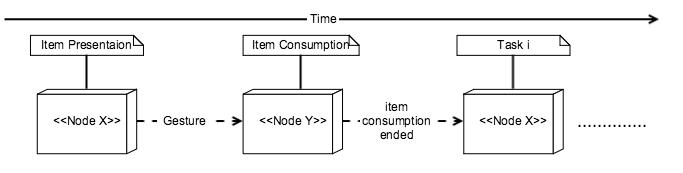
\includegraphics[width=0.9\textwidth, inner, center]{generic1}
\caption{Migrating Item Consumption from Presentation Node to Consumption Node.}
\label{fig:figure31}
\end{figure}

\subsection{Performing Parallel Activities}
\begin{figure}[h]
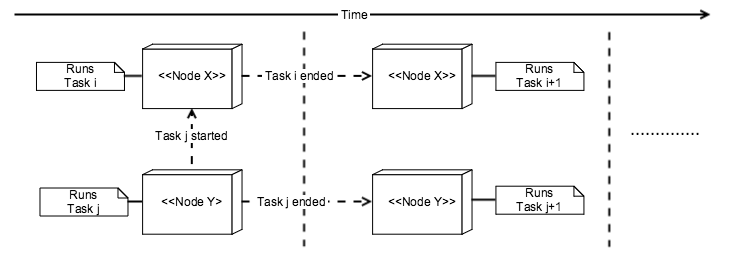
\includegraphics[width=0.9\textwidth, inner, center]{generic2}
\caption{Caption}
\label{fig:figure32}
\end{figure}
In a distributed environment, presenting the user with different platforms through which the user could perform tasks simultaneously could be leverage to perform parallel activities. In this case the distribution is achieved through distributing different interface components to be executed asynchronously (distribution in time). In contrast to the non-distributed scenario in which the user usually can not perform UI related tasks in parallel (asynchronously), but would usually wait for a UI task to be done before he/she could start the next (synchronously). Figure \ref{fig:figure32} is showing how a task could start running on a given node in the distributed environment, denoted here by task j on node Y, which triggers task i to start on node X. In this case, tasks are run in parallel and the user can perform these activities independently from each other and simultaneously. This is a case of distribution in time. After the tasks end on their given node, execution of proceeding tasks could be carried out also in a distributed manner. 
\subsection{Overview And Detail Presentations}
In a distributed environment with multiple displays, LD-SD modes are used to show different versions of the presented content to the user. There is always a concern on using different modes of what to choose to present to the user on which display/mode and what would be the basis for this choice. There is also the question of how to present the content differently on each mode based on its capabilities. Figure \ref{fig:figure33} suggests presenting a detailed presentation  of content on the SD on which the user could get all available detailed information of the provided content (for example in a form of a detailed list), while on the LD, the user could be presented with an overview of the same content (for example, in the form of picture icons with titles presented with in different sizes). Selecting an item on either mode later could lead to the execution of a proceeding task on either platform such as item consumption or viewing more information for the item.      

\begin{figure}[h!]
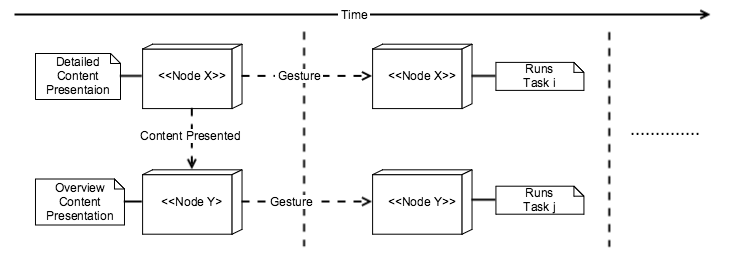
\includegraphics[width=0.9\textwidth, inner, center]{generic3}
\caption{Overview-Detail Presenations}
\label{fig:figure33}
\end{figure}


\subsection{Content Filtering}
As the user is presented with a wide array of recommended content, he/she might be willing to filter his/her choice of what to consume of this content. On a multi-device/platform environment, the filtering task could be distributed along the different nodes of the system. As shown in figure \ref{fig:figure34}, the user could initiate a gesture on items on node X to be transferred/redirected to node Y. By the end of this process, the user ends up with a presentation of all the selected/filtered items on node Y. The user could next select one of these items to view more details. This is an example of synchronous task distribution along different platforms.
  
\begin{figure}[h!]
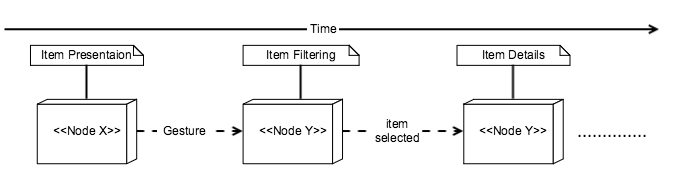
\includegraphics[width=0.9\textwidth, inner, center]{generic4}
\caption{Recommended Content Filtering}
\label{fig:figure34}
\end{figure}

\subsection{Content Redirection}
Content (output) redirection is a key feature in a multi-device environment [cite]. It is argued to be more important in case of multi-user systems, however, it could still be leveraged for single-user scenarios. Item consumption redirection is considered one special case of content redirection. Other examples would be redirecting recommended content details to be presented between SD and LD displays. Figure \ref{fig:figure35} shows how node X presents the recommended content, while on performing a gesture on any of the items, this content could be transferred/redirected to be presented on node Y. This usually means the distribution of UI components representing this content is what enables the redirection of content seamlessly between the two presentation nodes. The user could possibly then proceed with item consumption on the same node or on a different node.   
\begin{figure}[h!]
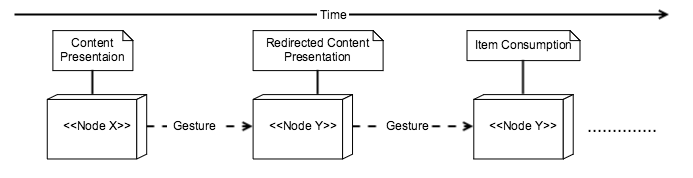
\includegraphics[width=0.9\textwidth, inner, center]{generic5}
\caption{Content Redirection}
\label{fig:figure35}
\end{figure}
\section{Design for a Single-User Video Recommender System in a Distributed UI Environment}
The proposed design is for a single-user, multi-device video cast recommendation application, in which the user interface and recommendation subtasks are distributed along the devices. The goal of the design is to leverage the capabilities of the distributed UI environment in order to find a new way to present the recommendation tasks and results to the user. In this section, we show how the recommendation tasks such as presenting the recommended items, item consumption, item rating, and others could be done in a distributed fashion. Our design is mainly targeted at benefiting from both platforms to make the post-recommendation phase of such system more efficient and more user-centric.
\subsection{Distribute for Whom?: UI Distribution In a Single-User System}

Our goal is the UI distribution of a single-user recommender system. The case for UI distribution of group recommenders in a multi-user environments has been made by a number of studies [cite]. The group recommendation involve multiple users with multiple devices. And since the main goal of a group recommendation is to reach consensus about a recommendation, distributed UI components that could be shared among the group members to reach this consensus is needed.

Less research have been made to make a case for the use of UI distribution of for single-user recommender systems. In such system, since a single user is involved in the process, and the consensus activity does not exist, it could be more challenging to think of what the distribution could be useful for in a single-user scenario. The main question on designing for such a system is to answer the question of why a single user would need a distributed environment; one with multiple devices and platforms. Why and if the action of recommendation for a single user with its various phases could be carried out on multiple devices/platforms, and whether the overhead(refer to the overhead described in earlier chapter) of distribution such a system is of an added value. The main challenge would be the introduction of a distribution mechanism for this system in such a way that does not hinder the process, and that would actually serve it. Also, the distribution should be done in such a way that does not introduce an overhead of shifting the user's attention from one platform/device to the other. 

\subsection{Platforms and Environment}
\begin{figure}[h!]
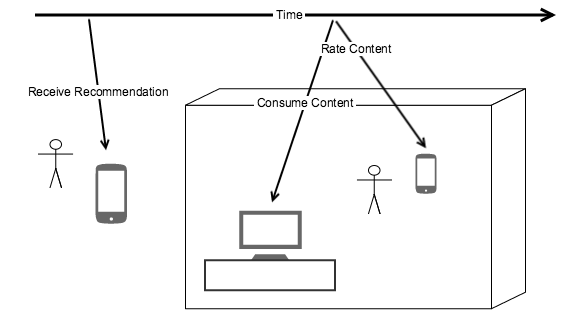
\includegraphics[width=0.6\textwidth, inner, center]{env}
\caption{Overall view of the system's environment}
\label{fig:figure311}
\end{figure}
To address some of the challenges mentioned in the previous section about designing for single-user in a distributed UI environment, we started by thinking of a scenario in which the user would be in need of, or would prefer to, use multi-devices to carry out the recommendation tasks. This lead us to think of a scenario that would start in a mobile environment. Figure \ref{fig:figure311} describes how the user receives recommendation for a new video cast on his/her mobile device while for example in commute. Since video content is usually lengthy and would be better viewed on a larger display than the limited space available on a mobile device display, the consumption of this content is thought to be better migrated to a large display device. The user could then migrate the consumption of this content to the LD once he/she reaches the environment that contains the LD (office, home, etc..). The application would then continue to operate in SD-LD mode; i.e. distributed among the mobile device (SD) and an LD, such that the user would be able to watch the video on the LD. In the following section, the distribution of video consumption as well as other recommendation subtasks are described.          
\subsection{Recommendation Tasks in a Distributed UI Environment}
In this section, the concept behind the distribution of pre and post recommendation tasks is provided. The reason for which tasks or UI components are selected to be displayed on which display, as well as the description of other distribution dimensions, are given.
\subsubsection{User Profile Creation}
The pre-recommendation phase usually starts by the elicitation of a user profile. Creating a profile usually involves filling out information forms, and likely rating some prototype items or entering preferences. This step would differ from one system to the other. For the video recommender, this involves asking the user directly to enter basic information and to rate a list of topics and interests to give a background about the user's preferences. 
The assumption in this step is that filling out textual forms as well as rating would better be performed on the handheld device than a larger display. The user is assumed to have more control over input for smaller devices. Therefore, this task starts at in the SD. As shown in figure, after the user finishes the profile creation step on the SD, the recommended content is then displayed on both SD and LD displays.
\begin{figure}[h!]
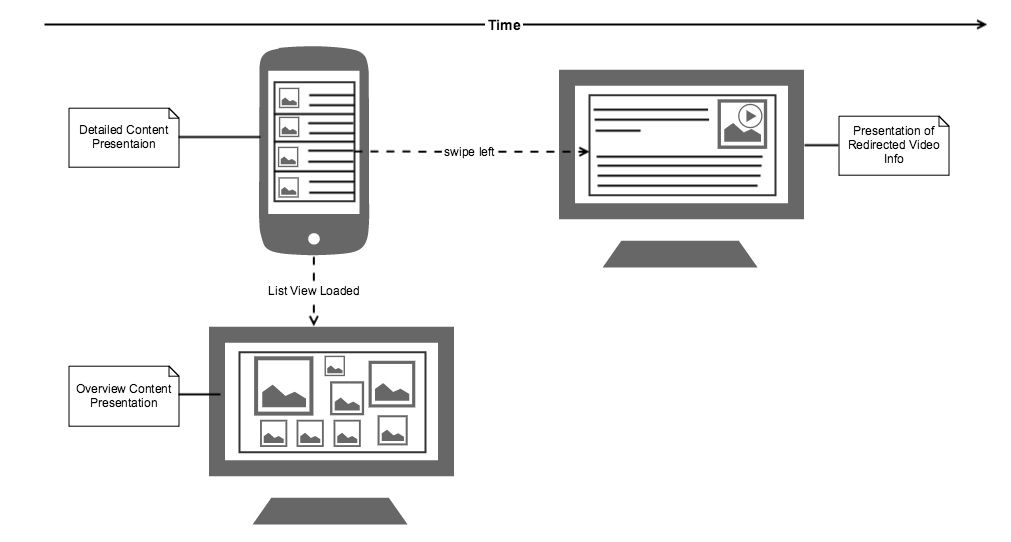
\includegraphics[width=0.85\textwidth, inner, center]{presentation-detail}
\caption{Presentation of Recommendation Results in LD-SD Modes.}
\label{fig:figure38}
\end{figure} 
\subsubsection{Presentation of Recommendation Results}
The presentation of recommended video casts is shown in parallel on the SD and LD, however, in different formats. We propose to present the recommended content at a different level of granularity for each platform; fine granularity is offered on the mobile device while coarse level of presentation is provided on the LD. As shown in figure \ref{fig:figure38}, for the mobile device, a detailed list of all the recommended videos, together with detailed information about the video, are shown in tabular form with different categorization. On the LD, an overview presentation is shown for the recommended items that scored the highest for the user without details, however shown in different sizes to indicate the recommendation score.
This way, we provide the user with alternative ways to view the content. At a glance, he/she could get an overview of the provided content with a graphical indicator for the recommendation score. Then, if more details is needed, the mobile device would provide more a detailed information about the video content. This concept UI distribution is what comes to be known as overview-detail coupling [cite].\\ 
For presenting the user with detailed information about the recommended videos, the recommendation list offers a link to a detailed information page on the mobile device in a master-detail fashion. As the user clicks on the item in the list, the user enters the detailed information page on the mobile device. Alternatively, as shown in figure \ref{fig:figure38} content redirection is also possible for viewing such information on the LD. Also by applying a simple swipe-right gesture on any of the video items in on the SD list, the video details content will be redirected to be displayed in parallel on the LD.   
    
\subsubsection{Recommended Item Consumption}
Playing the recommended videos is done as depicted by figure \ref{fig:figure36}. On the video details page, the user performs a pan gesture on the video image,  which then triggers the migration of the video consumption from the mobile device to the LD. The video player automatically stars on the LD, providing the user with all controls for the video playback.  
\begin{figure}[h!]
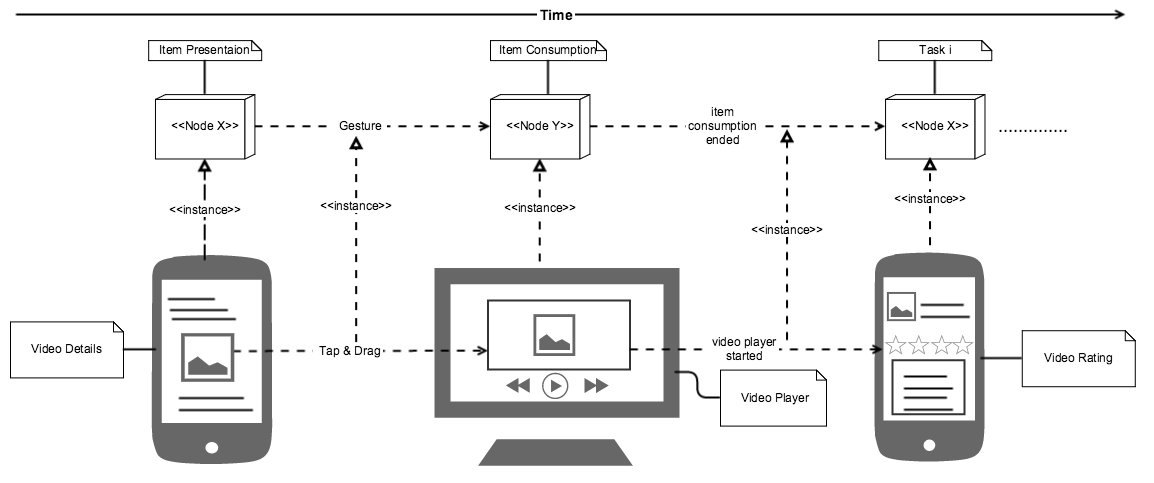
\includegraphics[width=0.9\textwidth, inner, center]{playrate}
\caption{Recommended Items Consumption.}
\label{fig:figure36}
\end{figure}
\subsubsection{Rating of Recommended Items}
There are two different proposed options for the rating task. The first option is distributed in time; i.e. done in parallel with the video playback. As shown in figure \ref{fig:figure36}, after the video playback starts automatically on the LD as described in the previous section, the LD triggers the mobile device to display the rating page for the user on the SD. Hence, the two tasks could be carried out simultaneously by the user.
Alternatively, the user could also be triggered to enter the rating on the mobile device after the video has ended playing or if stopped by the user on the LD. In such case, there is no parallelization of the tasks, however there is still synchronisation between the tasks that are carried out synchronously on the different platforms.\\
The rating, similar to the user profile creation, include user input such as indication of likes or entering textual comments and reviews, which is also believed to be best done on a mobile device with a better controlled input, for the user's convenience.  

\subsubsection{Filtering Recommended Items}
The filtering for the recommended items, although not a main task in recommendation, is believed to add to the value of the system in the proposed distributed UI environment. It is one of the tasks that leverages from the availability of the different platforms for the benefit of the user's experience. As shown in figure \ref{fig:figure39}, the filtering is done by performing a left swipe gesture on the video item in the list view on the mobile device.
\begin{figure}[h!]
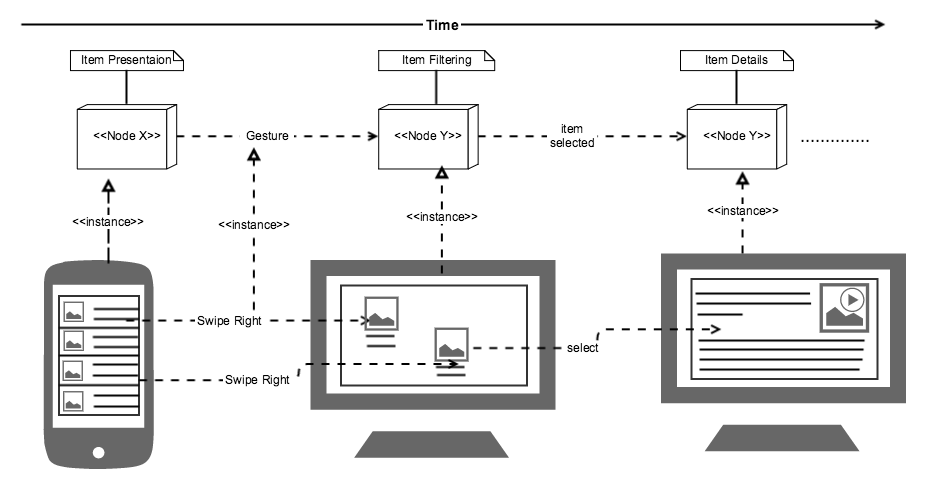
\includegraphics[width=0.85\textwidth, inner, center]{filtering}
\caption{Filtering of Recommended Items.}
\label{fig:figure39}
\end{figure}
This gesture redirects the content of the video to the LD. The display of the content on the LD is also done in a overview-detail coupling manner as described in earlier section. After the user is done filtering (redirecting selected content from SD to LD), LD will contain all the selected items displayed in an overview fashion. More details could be access through the SD or by also clicking on the item on the LD.  

\subsection{Transferring Recommendation Lists}
-Example of distribution initiated by user... (basically any type of content redirection)\\
-Select which components within a view (details view) are to be distributed.\\
-Readjust to old view after that
-Save as a configuration
-Rating: in parallel or after player?

\subsection{Pre-Configuring the System}
Meta UI. Time distribution. Enables system to load components differently at runtime. Select a configuration. Selecting which views to show on which platform.  

 
\chapter{Implementation of a DUI Video Recommender
Prototype}\label{chapter:impl} 
In chapter \ref{chapter:design}, a conceptual design for a single-user video recommendation application in a distributed UI environment was introduced. 
The goal of this design is to improve the recommendation process by leveraging
the capabilities of the different platforms along which the UI is distributed. To put the design to test, DiRec; a high-fidelity DUI video recommender prototype, was developed to mimic the functionalities of the complete system,
hence, making it possible for evaluation through a real user experience. We also
developed MiRec as a monolithic, non-distributed mobile video recommender. A
subset of the suggested distribution aspects with respect to the different distribution dimensions (user, task, time, space..etc) which was presented in the design chapter is selected for implementation.
The selection criteria of the scenarios to be implemented was the verifiability
of the scenario using our user study setup.
Since our user study involves only single-user scenarios, scenarios that need
more than one user at a time to verify (such as distributing a favourites list between users) were left out from the implementation.
Moreover, our focus is the distribution of the post-recommendation phase.
Consequently, tasks and activities involved in the pre-recommendation phase are
not implemented.
A recommendation engine is also not included since the focus of the study is not
recommendation generation. Instead, we provide the user with a set of
pre-selected video items.\\ 
This section provides the set of functionalities included in DiRec, as well as
an explanation of implementation details, together with explanations for the
rationale behind using the frameworks, programming languages, platforms and
tools used in the course of implementation.
 
\section{Functionalities of MiRec and DiRec}
As mentioned earlier, since the user study is designed to test whether the UI
distribution of such a system is of added value, the study is based on comparing user feedback on using two different versions of the prototype: a distributed
version (DiRec) and a non-distributed one (MiRec). This section explains the
difference between MiRec and DiRec through describing the different use cases of each version.
\subsection{Distributed Vs. Non-Distributed Use Cases}
The first steps of the design was to think of the different versions in terms
of user and system functionalities that would be available through each version.
MiRec and DiRec share similar functionalities, however, with different designs.
DiRec is distributed among a dual display (LD/SD), while MiRec is provided as a
mobile application. MiRec and the SD component of DiRec are implemented as iOS mobile applications.
In addition, DiRec has an LD screen component which is implemented as a
cross-platform python application. The iOS application in both versions are
fundamentally similar except for the use cases that were selected for distribution.
\begin{figure}[h]
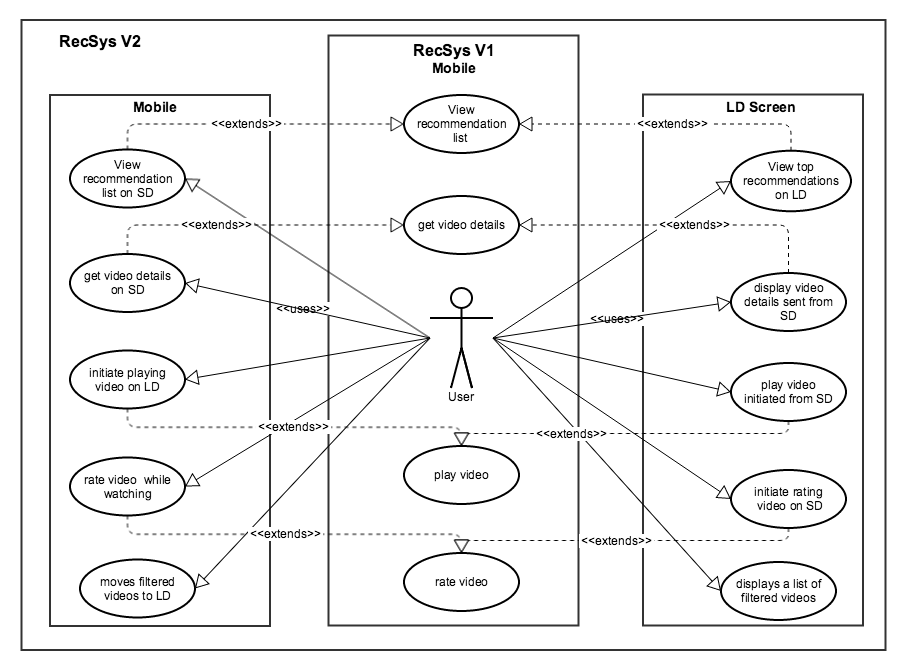
\includegraphics[width=0.8\textwidth, center, center]{figures/usecase}
\caption{Use Case Diagram of MiRec(RecSys V1) and DiRec(RecSys V2).}
\label{fig:figure42}
\end{figure}
As shown in figure \ref{fig:figure42}, the main use cases of MiRec are depicted
by the inner rectangle. They are described as follows:
\begin{itemize}
  \item The user should be able to view a list of all recommended videos. The list should be categorized with respect to the video topic or related topics.
  \item The user should be able to select a video and get more detailed
  information of the selected video.
  \item The user should be able to play the selected video on his/her mobile phone.
  \item The user should be able to rate the played video after watching.
\end{itemize}
The use cases of DiRec are given in figure \ref{fig:figure42} by the outer
rectangle and grouped by the SD/mobile and LD components of the system. The
functionalities are thought of as special cases, or extensions, of MiRec:
\begin{itemize}
	\item As opposed to getting a list of recommended videos on the SD, the user
	should be able to get both a list of recommend videos on the mobile phone (SD)
	as well as an overview of the top recommended video items on the LD. Both views should be presented in parallel one triggered by the other.
	\item Getting the video details should be available on the SD. Additionally, the user should be able to transfer the details of the video to be displayed on the LD using a simple gesture. 
	\item The video consumption/playing is distributed between the two displays. The user should be able to select the video on the mobile phone and with a simple gesture, should be able to trigger playing the video on the LD.
 \item Once the video starts playing on the LD, the user should be prompted with the rating view on the SD. Both functionaries (playing and rating) could be done in parallel.
 \item The user should also be able to filter his/her choices of videos. This use case is also distributed along both devices. The user should be able to apply a gesture on the selected video on the SD and get this video to be transferred to the LD. By the end of this process, the user should be able to be presented of all filtered videos on the LD. 
\end{itemize} 
The remainder of this chapter is dedicated to describe the implementation
details of DiRec. Since our focus is on the distributed UI scenarios
presented through DiRec, the implementation details of MiRec are not tackled.

\section{Overview System Architecture}
DiRec's dual-display system is composed of a mobile device application and an LD
screen application through which the interaction with the system is possible.
Figure \ref{fig:figure41} shows a deployment diagram of the different system components. The system is composed of two separate applications running on two different platforms with a communication layer between them: an iOS application running on an iPhone mobile device, and a python application running on PC connected to an LD screen.  A number of artifacts are needed to run both applications, as depicted by figure \ref{fig:figure41}: An iPhone mobile device with the .ipa of the mobile app installed on it, and on the LD side, a desktop application, with the Python runtime environment installed, should have the .py UI application installed on it. The PC is connected through an HDMI cable to an LD screen. Both the mobile device and the PC should be connected to the same network for communication.
    
This section provides implementation details of each application as well as the layer that channels communication between them.    
\begin{figure}[h]
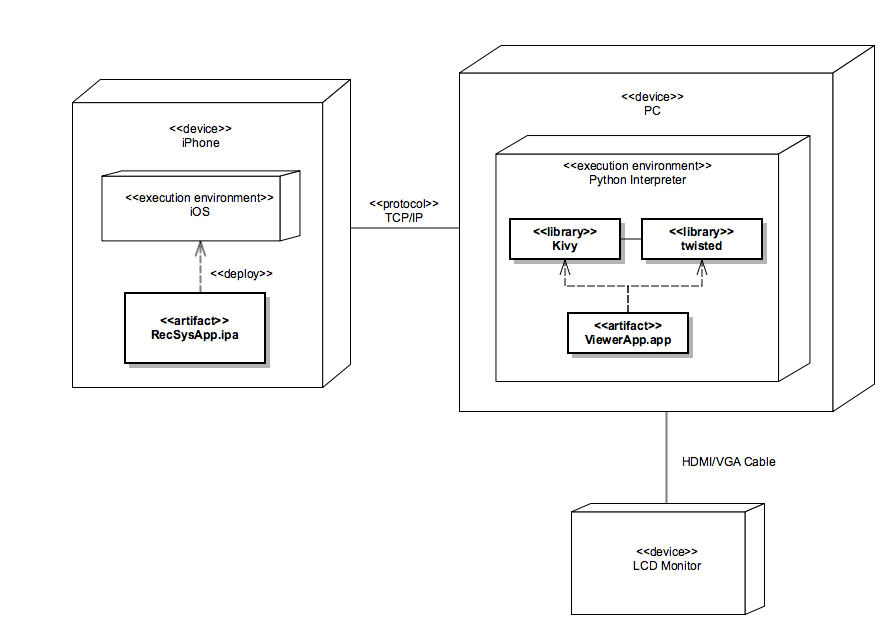
\includegraphics[width=0.8\textwidth, center, center]{figures/deployment}
\caption{Overview Architecture of The System's Components.}
\label{fig:figure41}
\end{figure}

\subsection{SD Mobile Application}
The first step of implementation, after deciding on the set of functionalities that should be present in each version as described in the previous section, was to start with creating a storyboard for the first non-distributed version of the application. As mentioned, the mobile application is implemented as a native iOS application running on iPhone mobile device. The app was written in Objective C, and uses Apple's iOS SDK 8.4 and basic frameworks for the implementation of most of the functionalities, except for some third party APIs that will be mentioned later. Xcode version 6.4 was used in implementing and preparing the distribution version of the app.\\
DiRec's SD component and MiRec did not vary with respect to the design of most
of the UI views and navigation options. Therefore, the
storyboard was not changed to a great extend from MiRec to DiRec. The main
variation was included on the level of functionalities implementation which will
be discussed in later sections.
  
\subsection{LD Screen Application}
The design of DiRec's LD application started by investigating the different
technologies available that support the functionalities we needed to implement
as a desktop application with a graphical UI. What needed to be supported was
means to build a graphical UI that enables user interaction, as well as the
capability of playing and controlling video files. Axiomatically, easy means for
communicating with the iPhone app that would allow for implementing the UI
distribution is a key feature. At first, implementing a Mac OS X desktop
application seemed as the best option. However, we refrained from using this
option as we aimed at a more portable option that also supports rapid prototype
development. Hence, a Python-based application was rather considered for
providing a more portable and light-weight solution for the development of this
special purpose prototype. Consequently, for the implementation of the desktop
application, we use Kivy \cite{kivyDoc}; an open-source Python-based library that was
developed with the creation of innovative user interfaces and rapid development as its primary edge. Kivy provides the tools needed to build graphical UI within its basic library, as well as libraries needed for video playback. The graphics engine is built over OpenGL ES 2, using a fast graphics pipeline. It also supports third party libraries that would be easily integrated for network communication with the iOS application as described in the following section. Kivy's portability makes it possible to run the developed application on any platform: Windows, Linux, OS X, iOS Android, which provides a length of variety on the selected platform for deployment.
 
\subsection{Communication Layer}
The development of applications with distributed UI components among different
platforms is not made possible through special frameworks or tools. Therefore,
it is up to every application developer to build a solution that makes the
UI distribution requirements achievable. In our model, we rely on a
message-exchange protocol between the iOS mobile application and the desktop
Kivy application. This message exchange work as commands sent between the two
applications to execute certain tasks (e.g. play video, show details, etc ...). This communication needs to be light-weight and quick to prevent any latency. One of the design goals is to provide seamless distribution of the UI between the two displays, such that the user would be able to carry out the tasks as efficiently as if the task was not distributed in the first place. Hence, the network communication between the iOS application and the Kivy desktop application is chosen to done through socket communication over TCP/IP. The desktop application, besides running its main functionalities, also runs as a custom TCP server that listens to connections on a given TCP socket. The client in this scenario is the iOS application which initiates connection once the app is running on a specific port and IP address. Using TCP sockets for communication makes the implementation of the communication layer independent on a web server, which also means a freedom to choose the implementation language for the server. Moreover, using TCP sockets provides light-weight means for building a lean and efficient protocol for communication through which we could send exact messages that needs to be sent between the applications.\\
To build the network protocol and the custom server on the desktop side Twisted
is used. Twisted is a Python networking framework that makes network
communication easier than using Python's basic networking library. Kivy also
comes with built-in support for Twisted. On the iOS side, the CFStream API is
used to establish a socket connection and, with the stream object created as a result, send data to and receive data from the custom python server on the desktop side.

\section{Implementation of DiRec's DUI Scenarios}

This section provides details of the implementation of DiRec's high-level
functionalities. It is worth noting that the implementation of such scenarios
were taking place iteratively; some of the mobile application functionalities
were implemented and later modified as more
scenarios were added or changed. Also, the implementation of the server desktop
side was done in parallel to the implementation of the iOS side in a continuous
integration manner in order to ensure that both sides integrate correctly. It is
also worth mentioning that the data gathered for this prototype was done using a
Python script that scrapped TED.com for video cast files' urls and information
including detailed description, speakers, dates, images and duration. A total of
73 video casts' information was gathered from different topics. Data was not
saved in a database, however, was duplicated as XML-based property list files on
both the iOS and desktop sides. For the sake of rapid development of this
prototype, fast access of data was needed. Since the collected data fits a
dictionary representation and has no relational aspect, creating a separate
database was thought of as redundant. Moreover, the duplication of the property
list resource on both sides is considered a more efficient option than having
to access a shared resource despite of the update overhead that would be necessary if any of the copies were to be edited.\\
Appendix \ref{chapter:appendA} provide a high-level class diagram for both iOS
and LD desktop applications for more details.

\subsection{Establishing Connection}
Initialising TCP sockets communication between the iOS app and desktop app is
the initial step. Since the desktop LD application works also as the server,
this step has to start by calling Twisted reactor on the server side to start its main loop and
wait for connections from the iOS client. The specific IP address and port for
communication are hardcoded in the application for simplicity, so that no
pairing mechanism would need to be implemented. Once Twisted is started and
added successfully to the main loop of the Kivy application, the desktop app
enters the \textit{Waiting for Connection} state. Consequently, DiRec's LD
component's welcome screen is shown, which indicates that the server is running and
waiting for connection.\\
On the iOS application side, a Communication Manager singleton class is
initialised in the App Delegate once the application finishes launching. In the Communication Manager init method, NSStreams (input and output) are created after a connection with the server is requested at the given IP address and port which are also hardcoded with the same values as the desktop application. Once a connection is made successfully (given that the server is already running), Communication Manager initialises the messaging protocol with the following messages:
\begin{itemize}
	\item \textbf{\textit{open:home}} for opening home view on LD. 
	\item \textbf{\textit{play:<videoID>}} for playing a video with id \textit{videoID} on LD.
	\item \textbf{\textit{detail:<videoID>}} for redirecting details of video with id \textit{videoID} to LD.
	\item \textbf{\textit{filter:<videoID>}} for redirecting video with id \textit{videoID} for filtering on LD.
	\item \textbf{\textit{rate:<videoID>}} for rating video with id \textit{videoID} on SD.
\end{itemize}

As shown, the message payload consists of a command part and a value part
separated with a colon. In case video information needs to be redirected, only
the video id is sent and not the actual content of the video. This way, we
minimise the overhead of communication by passing light-weight messages that are
sufficient for performing the tasks. At this point, the desktop server enters
the \textit{Ready} State and awaits receiving messages from the iOS client.

\subsection{Loading Videos' Data}
After the connection is established successfully and the protocol is
initialised, loading of the videos' data is done on both sides. On the iOS side,
a data model class \textit{Video} is created to hold video details. For each
video object, the following attributes are loaded: id, title, description,
speaker, duration, year, and topic. The data is loaded in memory once from the
property list by a Data Manager as Video objects. On the desktop side, the property list is also loaded in a read-only list structure.

\subsection{Presentation of Recommended Videos}
The first distributed UI scenario that a user is presented with is the
presentation of a Home view which holds the recommended video items (Figure
\ref{fig:figure43}). On the iOS side, the videos are presented as a TableView
list, which also acts as a master view to a details view  which is loaded on
clicking one of the items. Fine granularity of detail is presented to the user
on the iOS side.
\begin{figure}[!htpb]
    \centering
    \begin{subfigure}[b]{0.6\textwidth}
        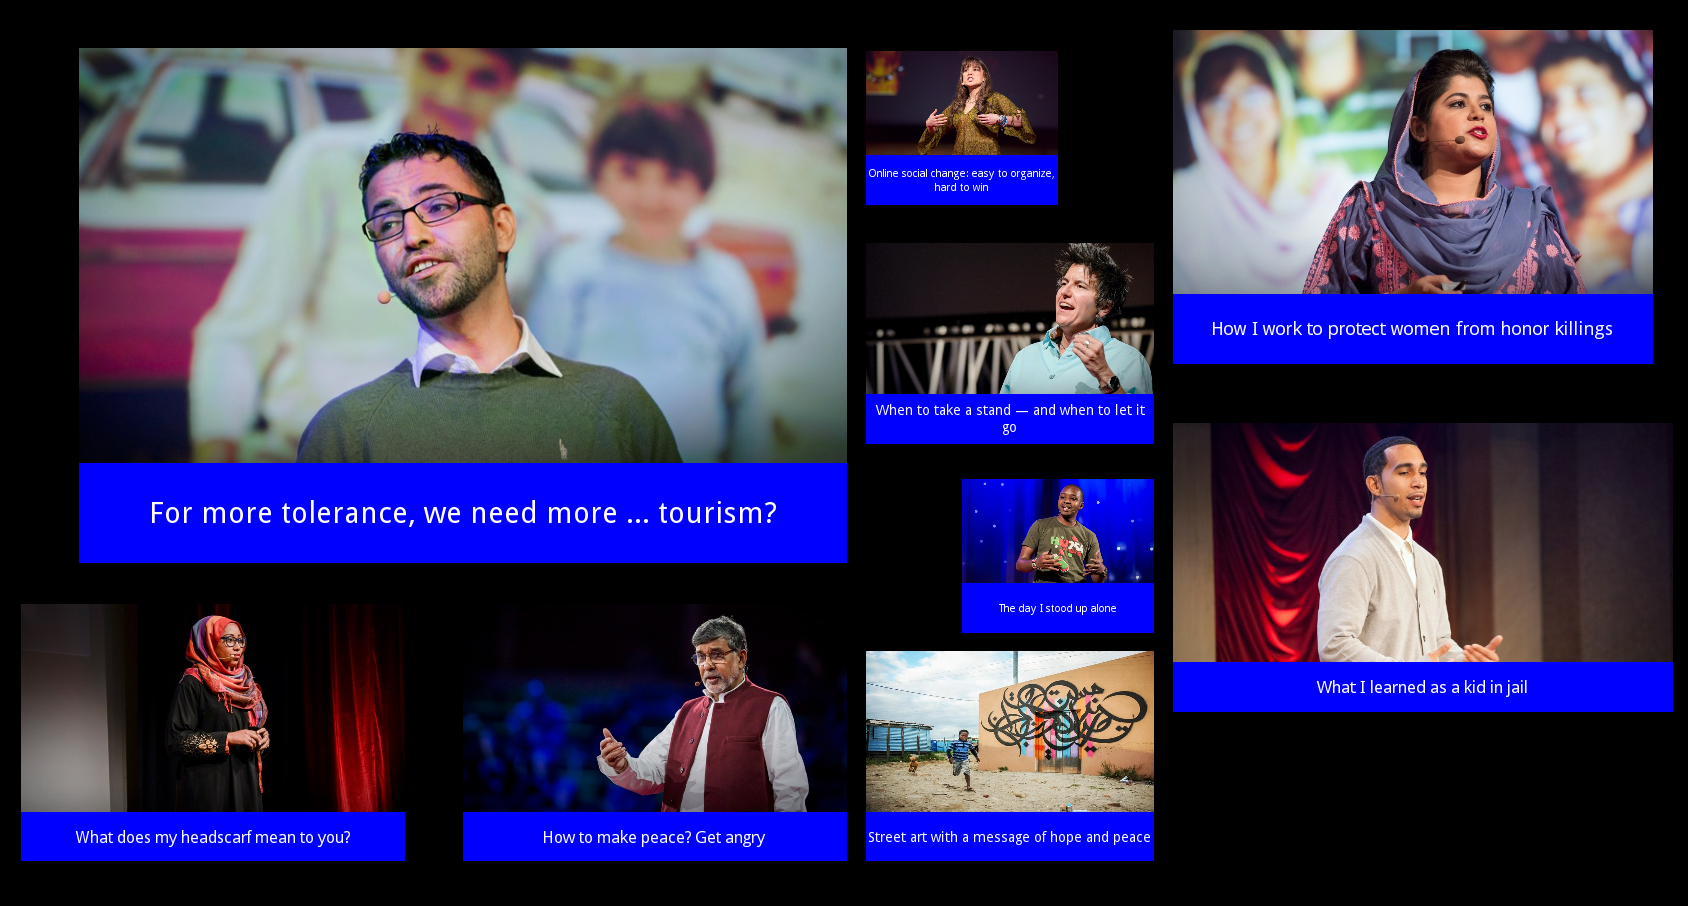
\includegraphics[width=\textwidth]{figures/homeLD}
        \caption{Home view on LD display.}
        \label{fig:figure43a}
    \end{subfigure}
    ~ %add desired spacing between images, e. g. ~, \quad, \qquad, \hfill etc. 
      %(or a blank line to force the subfigure onto a new line)
    \begin{subfigure}[b]{0.3\textwidth}
        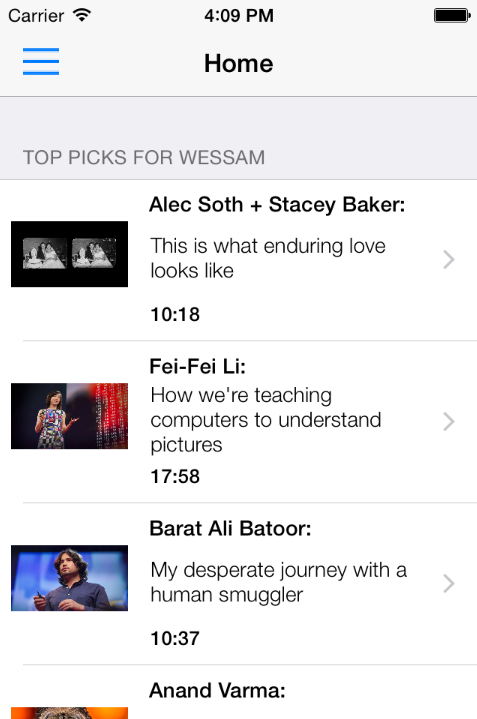
\includegraphics[width=\textwidth]{figures/homeSD}
        \caption{Home view on SD/mobile display.}
        \label{fig:figure43b}
    \end{subfigure}
   \caption{Presentation of Recommended Videos on SD and LD displays}\label{fig:figure43}
\end{figure}
The list is divided into sections showing different
categorisation titled with explanations as such: \textit{Top Picks for <User>},
\textit{Because You Liked <Category>}, \textit{Top Rated in <Category>}, \textit{You Might Also Like}, etc... This type of explanation is not based on actual recommendation logic but was added to mimic real recommendations. A side menu enables the user to get a list of all available categories for further details. Selecting one of the categories would also open a list view similar to that of Home however specific to that category.
Simultaneously, on loading the home view on iOS, \textbf{\textit{open:home}} is sent to the sever to load the home view on the desktop side. On receiving this message, the server loads a Grid layout with an overview presentation of recommended videos in different sizes which indicate the recommendation score.


\subsection{Presentation of Video Details}
Getting details of a video (Figure \ref{fig:figure44}) is started on the iOS
side by clicking on a given video in the Home list which presents a details view. The details view is
similar in both MiRec and DiRec. Additionally in DiRec, redirecting the details
of the video to the LD is possible by performing a left swipe gesture on the
TableView cell of the video item on the iOS side. After performing the gesture,
Communication Manager sends \textbf{\textit{detail:<videoID>}} with the specific
video id. The desktop server receives and parses the sent message. For the
command \textbf{\textit{detail}}, a layout is created, loaded, and filled with
the content of the video details the id of which was sent as the value part of
the parsed message. Hence, the user is able to view details of the videos on
both the SD and LD.
\begin{figure}[!htpb]
    \centering
    \begin{subfigure}[b]{0.6\textwidth}
        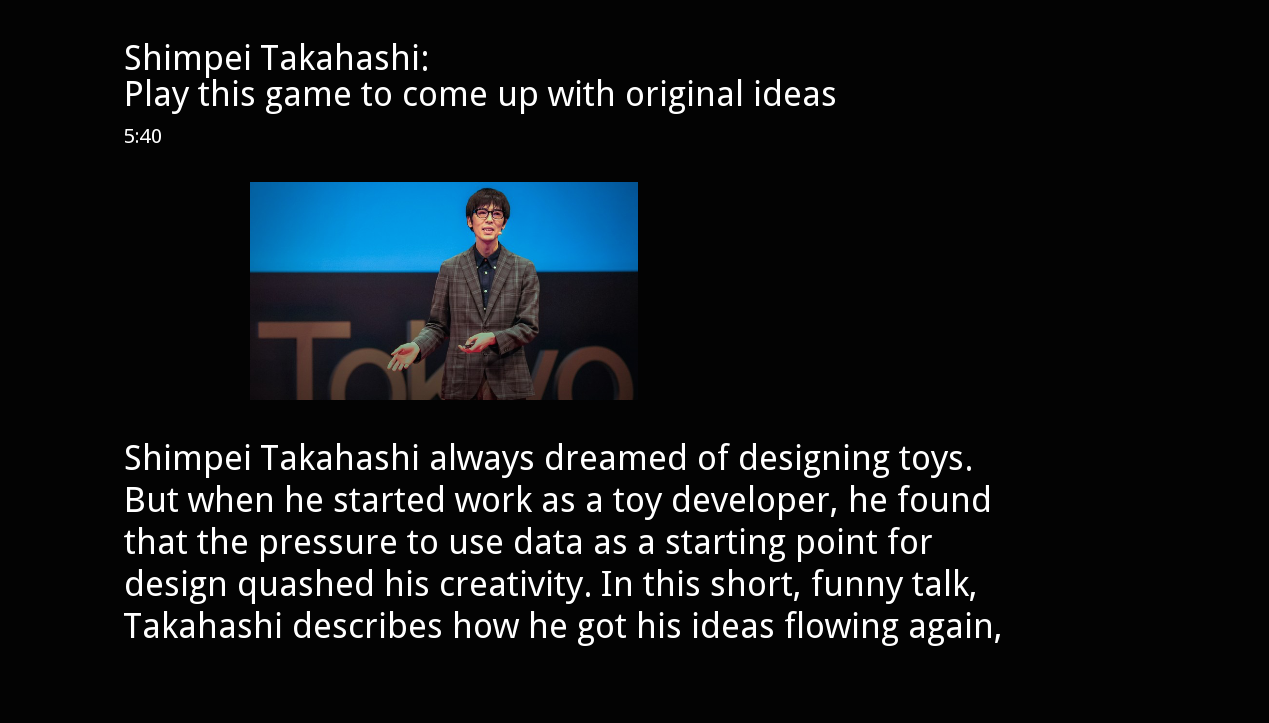
\includegraphics[width=\textwidth]{figures/detailsLD}
        \caption{Showing video details on LD}
        \label{fig:figure44a}
    \end{subfigure}
    ~ %add desired spacing between images, e. g. ~, \quad, \qquad, \hfill etc. 
      %(or a blank line to force the subfigure onto a new line)
    \begin{subfigure}[b]{0.3\textwidth}
        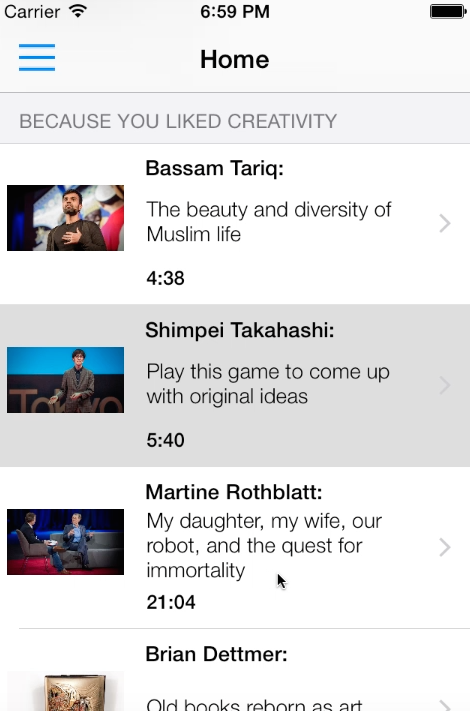
\includegraphics[width=\textwidth]{figures/swipeleftSD}
        \caption{Swipe-left gesture on table view cell.}
        \label{fig:figure44b}
    \end{subfigure}
   \caption{Presentation of Video Details}\label{fig:figure44}
\end{figure}
\subsection{Playing a Video}
The distributed scenario of playing a video (figure \ref{fig:figure45},
\ref{fig:figure46a}) is one that also starts at the iOS side. The user select a
video from the list and then is directed to a details page. Inside the details
page, besides viewing the video's details, to play a video on the LD, the user
simply taps and drags (panning) the image of the video presented in the centre
of the screen towards the bottom of the screen. Figure \ref{fig:figure45a} shows a sample
of this action. The panning gesture triggers sending a message to the desktop
server \textbf{\textit{play:<videoID>}}, which sends the play command and the selected video id to the server. The server receives and parses the message and loads an instance of a video player initialized with the video url. The video player starts streaming the content and displaying it on the attached LD screen. For playing and controlling the video kivy.uix.videoplayer package is used which is built-in in the Kivy library.\\
In the non-distributed scenario, MiRec presents the user with a play button on
top of the video image in the details page. On clicking the button, the video player is loaded as a modal view on top of the details view, where control and playing of the video is made possible on the mobile device.
\begin{figure}[!htpb]
    \centering
    \begin{subfigure}[b]{0.3\textwidth}
        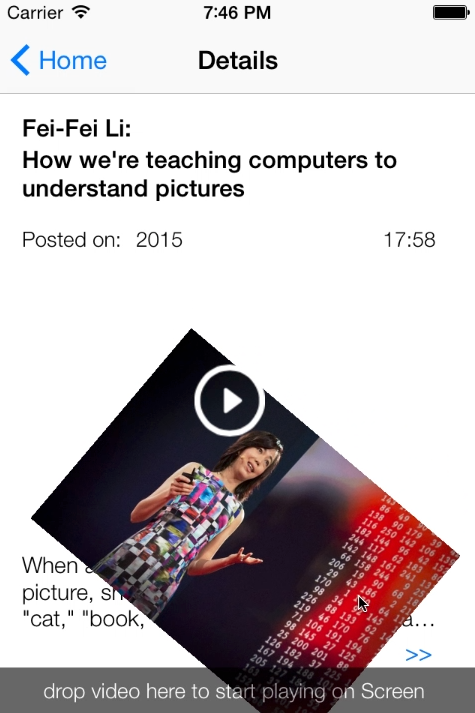
\includegraphics[width=\textwidth]{figures/playSDb}
        \caption{Pan gesture on video image}
        \label{fig:figure45a}
    \end{subfigure}
    ~ %add desired spacing between images, e. g. ~, \quad, \qquad, \hfill etc. 
    %(or a blank line to force the subfigure onto a new line)
    \begin{subfigure}[b]{0.3\textwidth}
        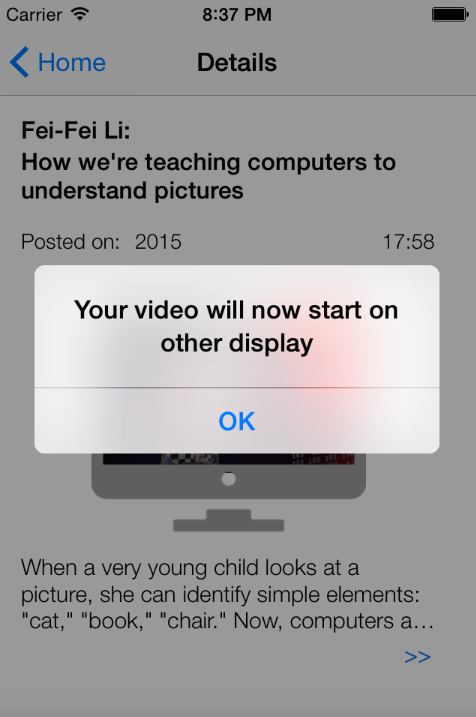
\includegraphics[width=\textwidth]{figures/playSDd}
        \caption{Notification alert to play transfer video to LD.}
        \label{fig:figure45b}
    \end{subfigure}
    \begin{subfigure}[b]{0.3\textwidth}
        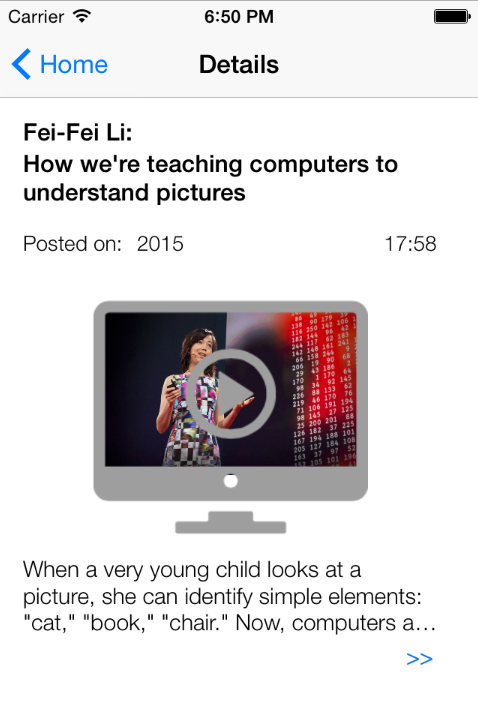
\includegraphics[width=\textwidth]{figures/playSDc}
        \caption{Indication that the video has started on LD}
        \label{fig:figure45c}
    \end{subfigure}
    \caption{Initiating video playing on LD}\label{fig:figure45}
\end{figure} 
\subsection{Rating a Video}
In the distributed version of playing a video, starting the rating scenario is done once the player is started on the LD. The desktop sever sends a message \textbf{\textit{rate:<videoID>}} to the iOS app to display the rating view. Hence, the user could perform both tasks (rating and playing) in parallel. Figure \ref{fig:figure46b} shows the rating screen on the iOS side.
The same screen is shown in the non-distributed version however it is prompted after video playing on the SD ends or is stopped by the user.

\subsection{Filtering Recommendations}
Optionally, the user is able to filter his/her choice of videos before deciding on which videos to play. 
Filtering is done by transferring the selected video from the recommendation list on iOS side to the LD application by performing a right swipe gesture on the video item table view cell. 
\begin{figure}
    \centering
    \begin{subfigure}[b]{0.6\textwidth}
        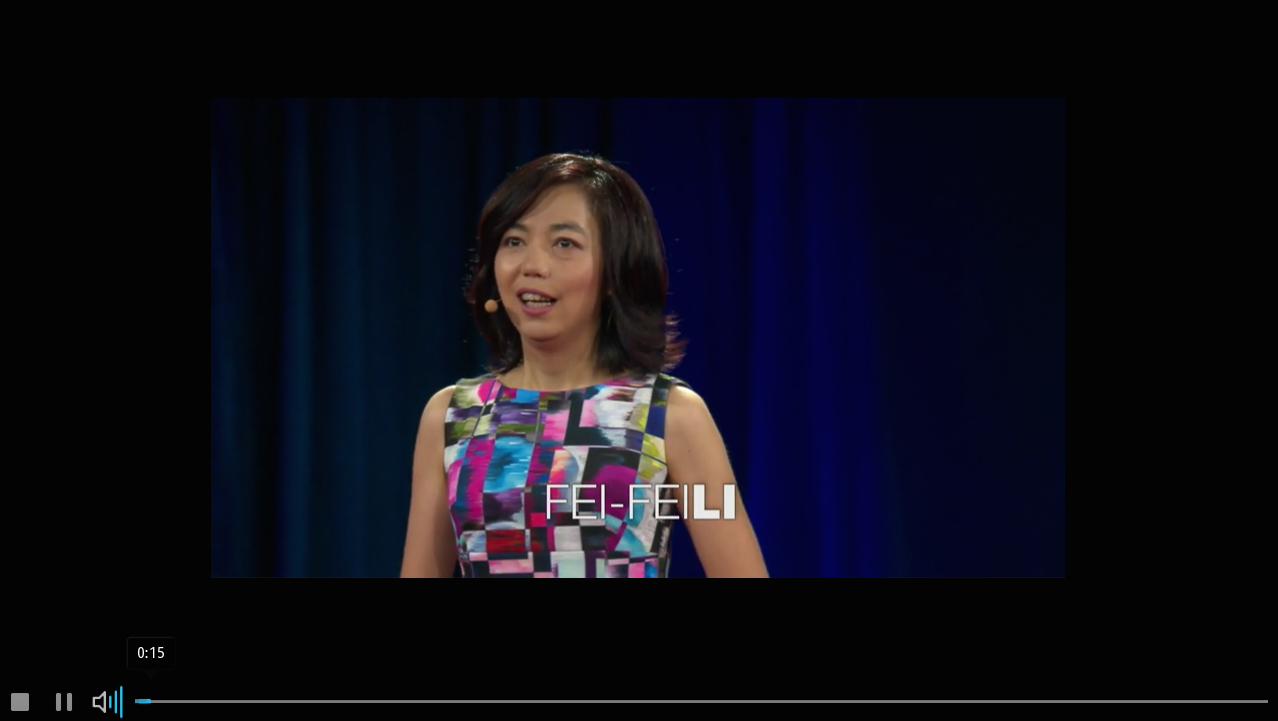
\includegraphics[width=\textwidth]{figures/playerLD}
        \caption{Video player started on LD}
        \label{fig:figure46a}
    \end{subfigure}
    ~ %add desired spacing between images, e. g. ~, \quad, \qquad, \hfill etc. 
      %(or a blank line to force the subfigure onto a new line) 
    \begin{subfigure}[b]{0.3\textwidth}
        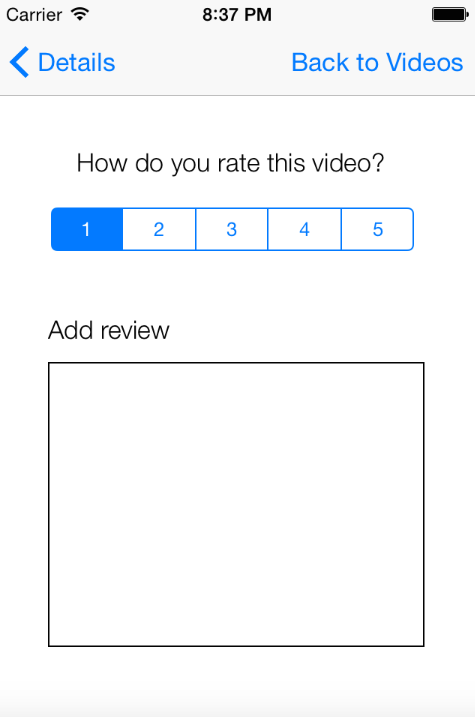
\includegraphics[width=\textwidth]{figures/ratingSD}
        \caption{Rating view started on SD on starting video player on LD}
        \label{fig:figure46b}
    \end{subfigure}
   \caption{Rating recommended videos on SD while playing a video on LD}\label{fig:figure46}
\end{figure}       
The swipe gesture triggers sending a message \textbf{\textit{filter:<videoID>}} from the iOS side to the desktop server side. 
When the message is received on the server side, the filter page is created as a
grid layout and each transferred video is added as a new widget to the layout.
Only the video image and title are shown on the LD. The user is also able to display more information for the page by clicking on the video image on the LD side. Figure \ref{fig:figure47} shows the filtering scenario as presented on the LD and SD.\\

 
In the next chapter, we are going to present the details of conducting a user
study in which DiRec and MiRec's functionalities were used and rated by a number
of participants, and how we evaluate and interpret the results of the study in
an attempt to evaluate the design of our presented DUI video recommender.
\begin{figure}[!htpb]
    \centering
    \begin{subfigure}[b]{0.6\textwidth}
        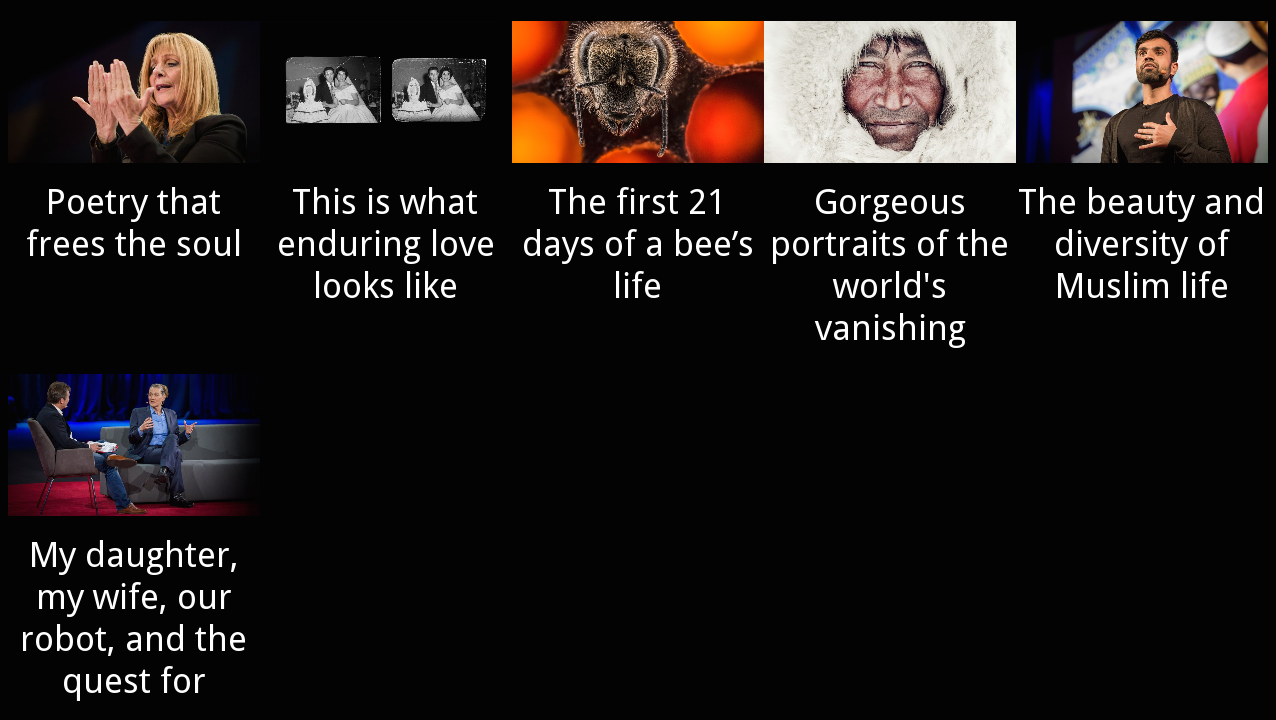
\includegraphics[width=\textwidth]{figures/filterLD}
        \caption{Filtering screen on LD}
        \label{fig:figure47a}
    \end{subfigure}
    ~ %add desired spacing between images, e. g. ~, \quad, \qquad, \hfill etc. 
      %(or a blank line to force the subfigure onto a new line)
    \begin{subfigure}[b]{0.3\textwidth}
        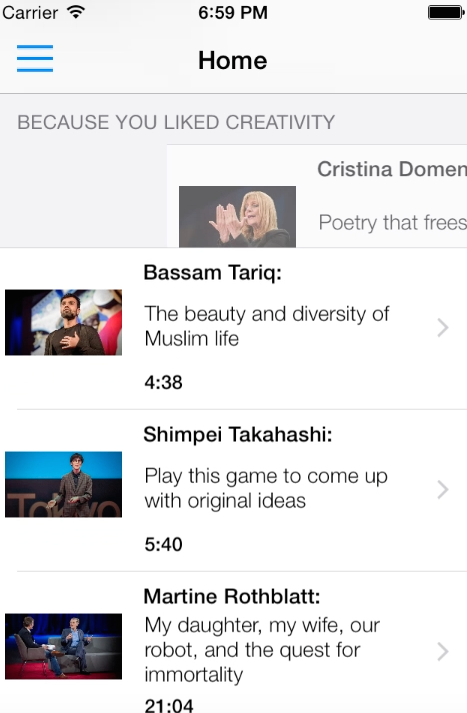
\includegraphics[width=\textwidth]{figures/swiperightSD}
        \caption{Right swipe gesture on table view cell on SD.}
        \label{fig:figure47b}
    \end{subfigure}
   \caption{Filtering Recommendations}\label{fig:figure47}
\end{figure} 
         



\chapter{Evaluation}\label{chapter:eval}
In previous chapters, we introduced the design and implementation of 2 prototype
video recommendation applications, MiRec and DiRec, that are developed for the
purpose of testing the effect of distributing the UI of a single user recommender system on the users'
experience; whether this distribution will enrich and facilitate users'
experiences of such systems or would be considered redundant or confusing. To
put this to test, we designed a closed user study, in which participants were
asked to interact with and use both prototype applications, and then give their
feedback evaluation through a user experience survey directly after they are done with
using the apps. In this sections, we explain the different phases of the user
study. We also explain our evaluation method, as well as present the results of
the analysed user experience survey collected from the study participants.

\section{User Study Phases}
The overall goal of the study is to elicit the users’ direct
feedback and impressions of their experience of using the prototype apps.
Each of the phases described below will have its own sub-goal that works
towards this main goal. The study is divided into 3 phases. It starts in a
usability demo in which we demonstrate to participants how to use the apps,
which we thought is necessary to avoid any confusion which might affect the
users rating of the app and tamper with their evaluations. Phase 2 is the actual
user test in which participants interact and use the apps. And the final phase
is the post-experiment user experience survey which is done shortly after phase
2. In the course of 2 weeks, participants were invited to use our apps and give
their feedback. We started our evaluation of the collected user feedback shortly
after we had sufficient number of participants that lead to a stable evaluation.
The following are details of each phase of the study as well as a presentation
of the results and how we interpret them.
\subsection{Phase 1: Usability Demo}
The goal of this phase is to explain clearly to participants the functionalities
of both prototypes. According to the participant’s background, information about
recommender systems, their goal and how they work, were provided. We started by
explaining to participants what tasks are expected to be completed by the them.
We explained that both apps function similarly except that with DiRec, some
functionalities could be done on the phone and others could be transferred to
the screen. We then proceeded with demonstrating to the participant what they
could do with each app. In MiRec, we explained how to play and rated videos, how
to view the video details, and how to navigated through the list of
recommendations in the Home screen as well as through the categories. In DiRec,
we also demoed what could be done on the phone and what could be done on the
screen. The gestures of swipe-left to view details on screen, swipe-right to
filter, and pan on video photo to play on screen were also demoed clearly so
participants would know how to perform the tasks. We explained that the goal of
the study is not to test the functionalities but to get their impression about
the apps. After all fucntionalities were demoed, participants were handed in a
sheet that has the tasks they are expected to complete written down in the form of steps (see appendix). Also, they were
handed in the user-experience questionnaire sheets. Participants were asked to
take their time and ask any questions if needed and to fill-in the questionnaire
directly after they are done.
\begin{figure}[t]
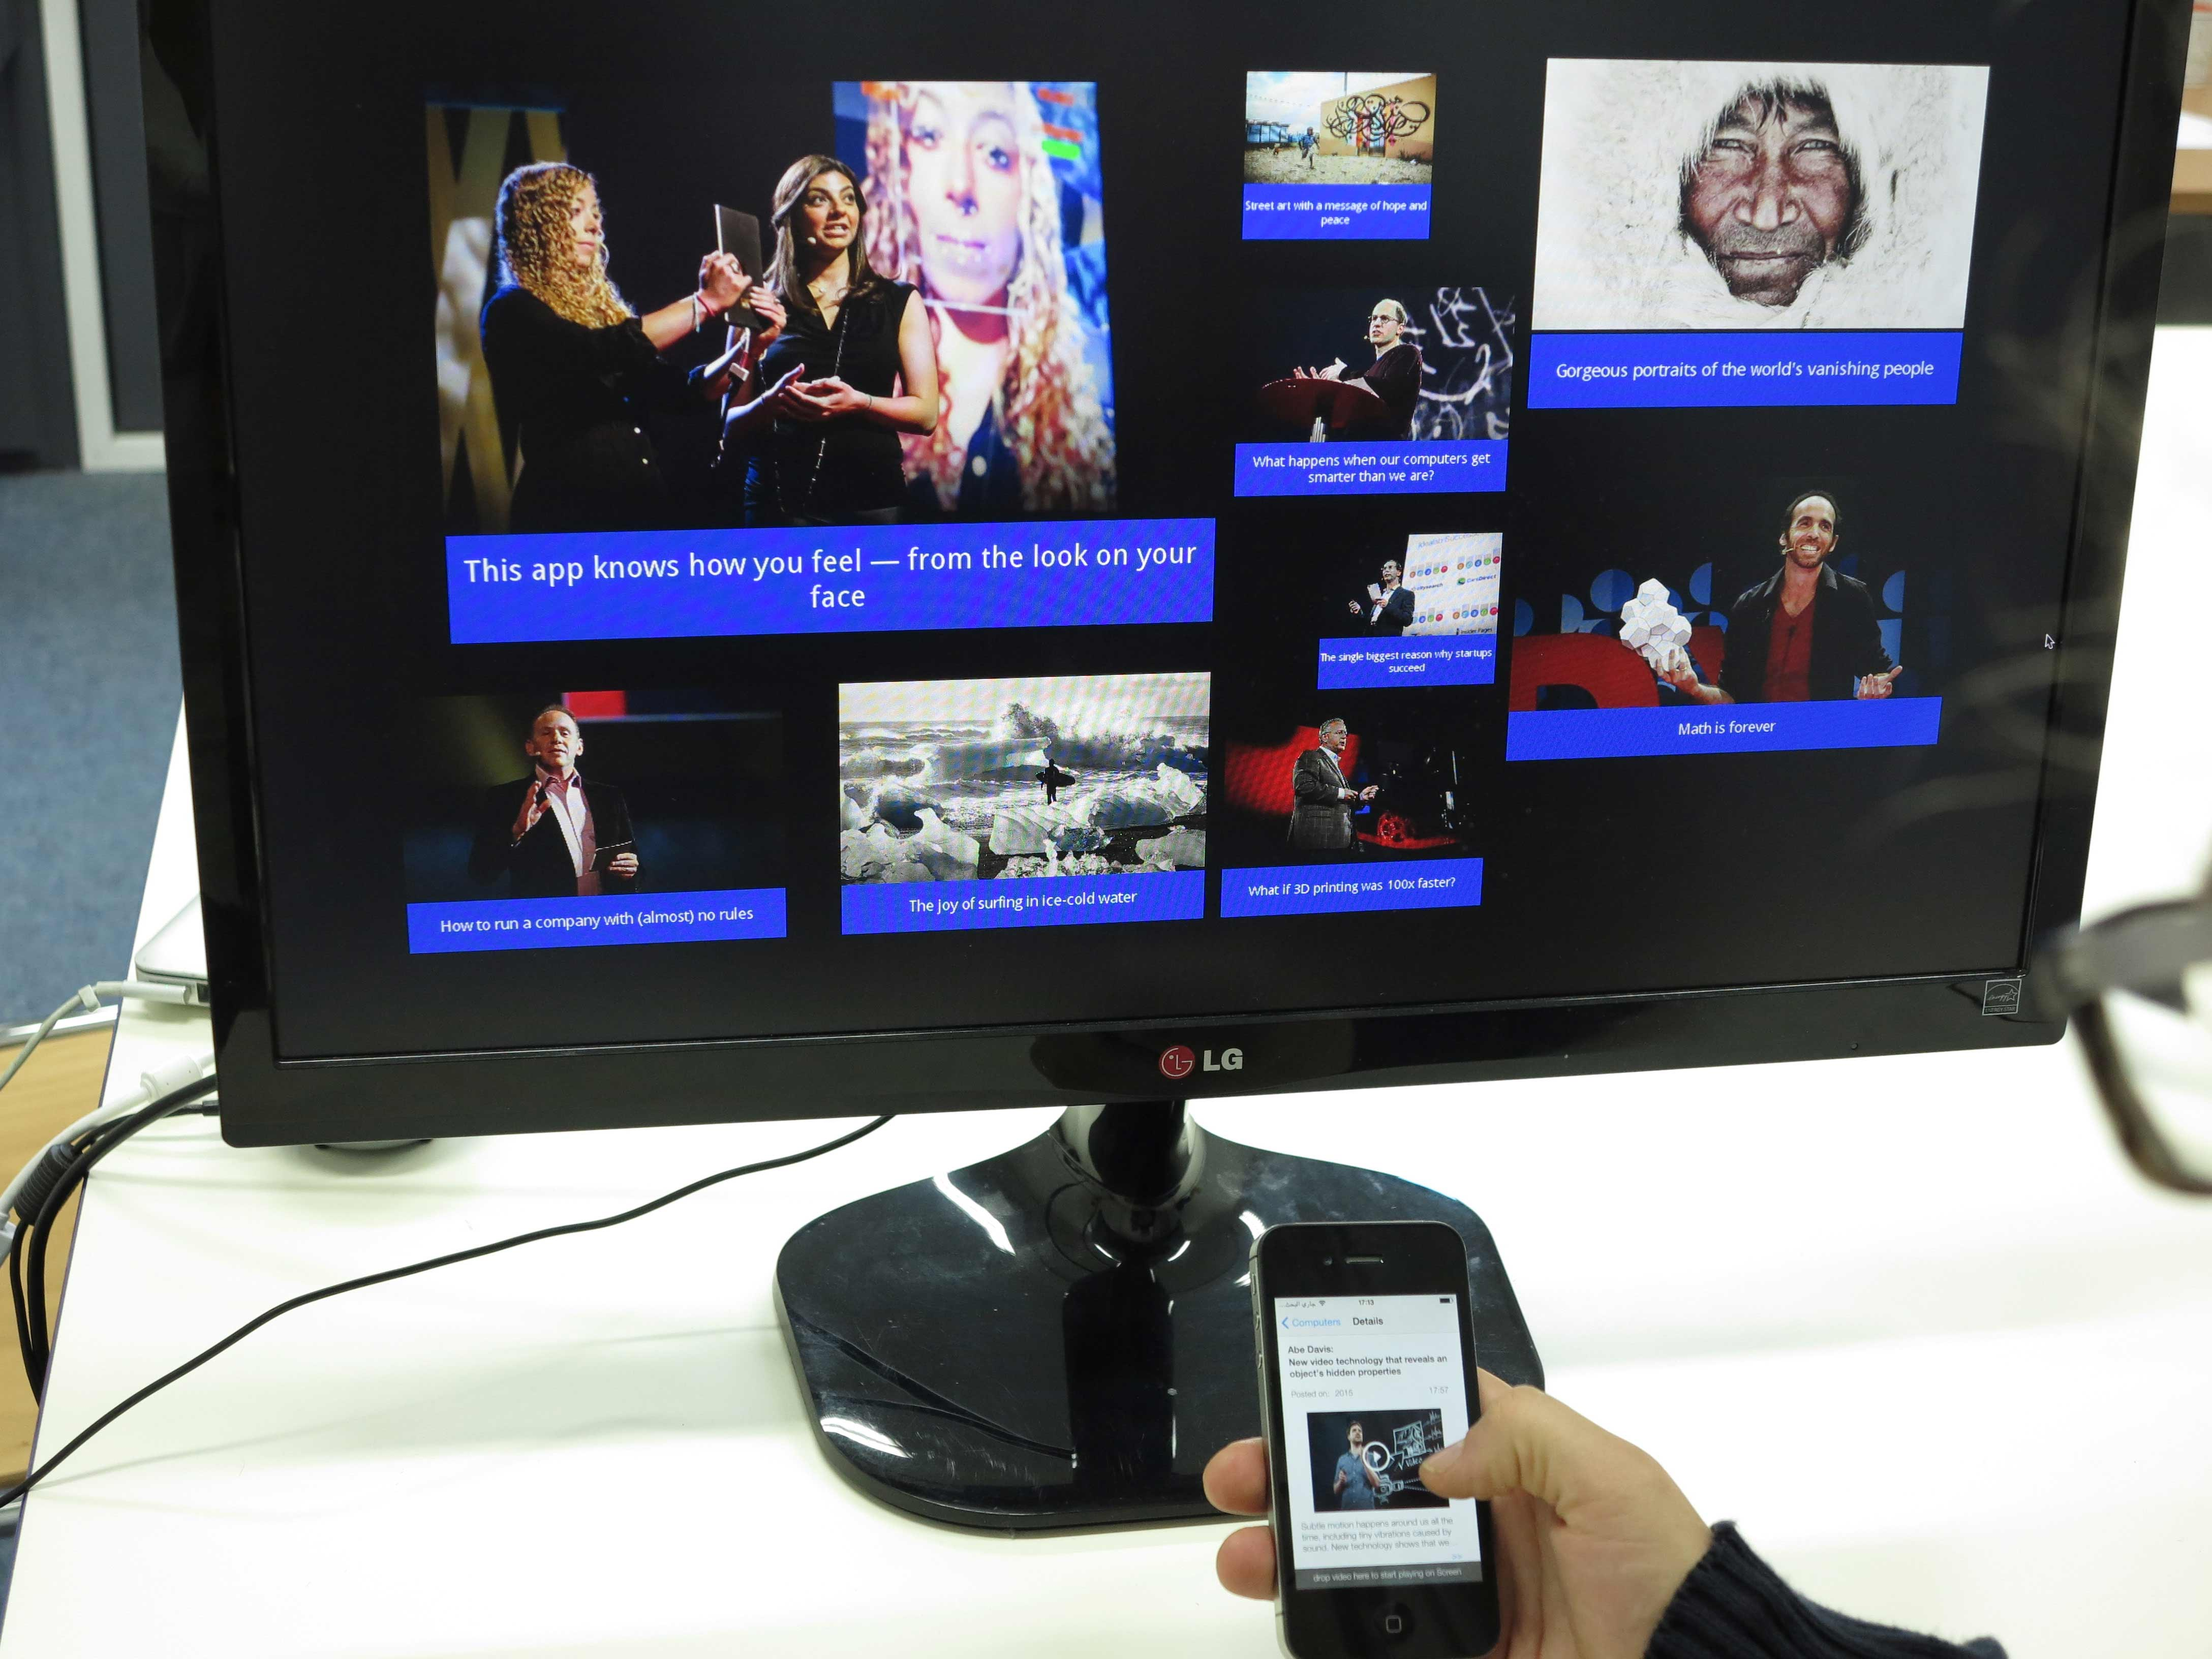
\includegraphics[width=0.75\textwidth, center, center]{figures/IMG_6806}
\caption{Participant's interaction with DiRec during the study.}
\label{fig:figure51}
\end{figure}
\subsection{Phase 2: Prototypes' Functionalities Test}
The user test was done after the participant was made familiar with the apps and
with the tasks of the study. Figure \ref{fig:figure51} shows part of one of the
participant's interaction with DiRec during phase 2 of the user study. Each
participant was given an iPhone mobile device with MiRec and DiRec installed, and was asked to sit across of an LD screen, which works as a display to DiRec's LD component.
Participants were asked to start with the app version of their choice to avoid
bias. After they are done with a given version, they start the tasks of the
second version. The tasks were put in place so as to have a standard set of
steps that all participants do. These steps (appendix) mainly consist of:
navigating the list of recommendations through the Home screen, viewing video details, playing
a video, rating a video, selecting a category of choice from the side menu, and
for DiRec, filtering was added to this list. By the end of each set of steps in
each app, we note that optionally users could then proceed interacting with the
apps for whichever scenarios they have in mind. Participants were informed that
this session would on average take between 15 to 20 minutes but they were also
asked to take their time or to stop the experiment at any time if they feel they
are already done and have a feel of the apps already formed. Participants were
observed during this test session, as part of the evaluation is to see how users react to the distribution aspect of the app.
Our observations of participants' interactions constitute part of our evaluation
of the results as shown later in the result section.
\begin{figure}
    \centering
    \begin{subfigure}[b]{0.3\textwidth}
        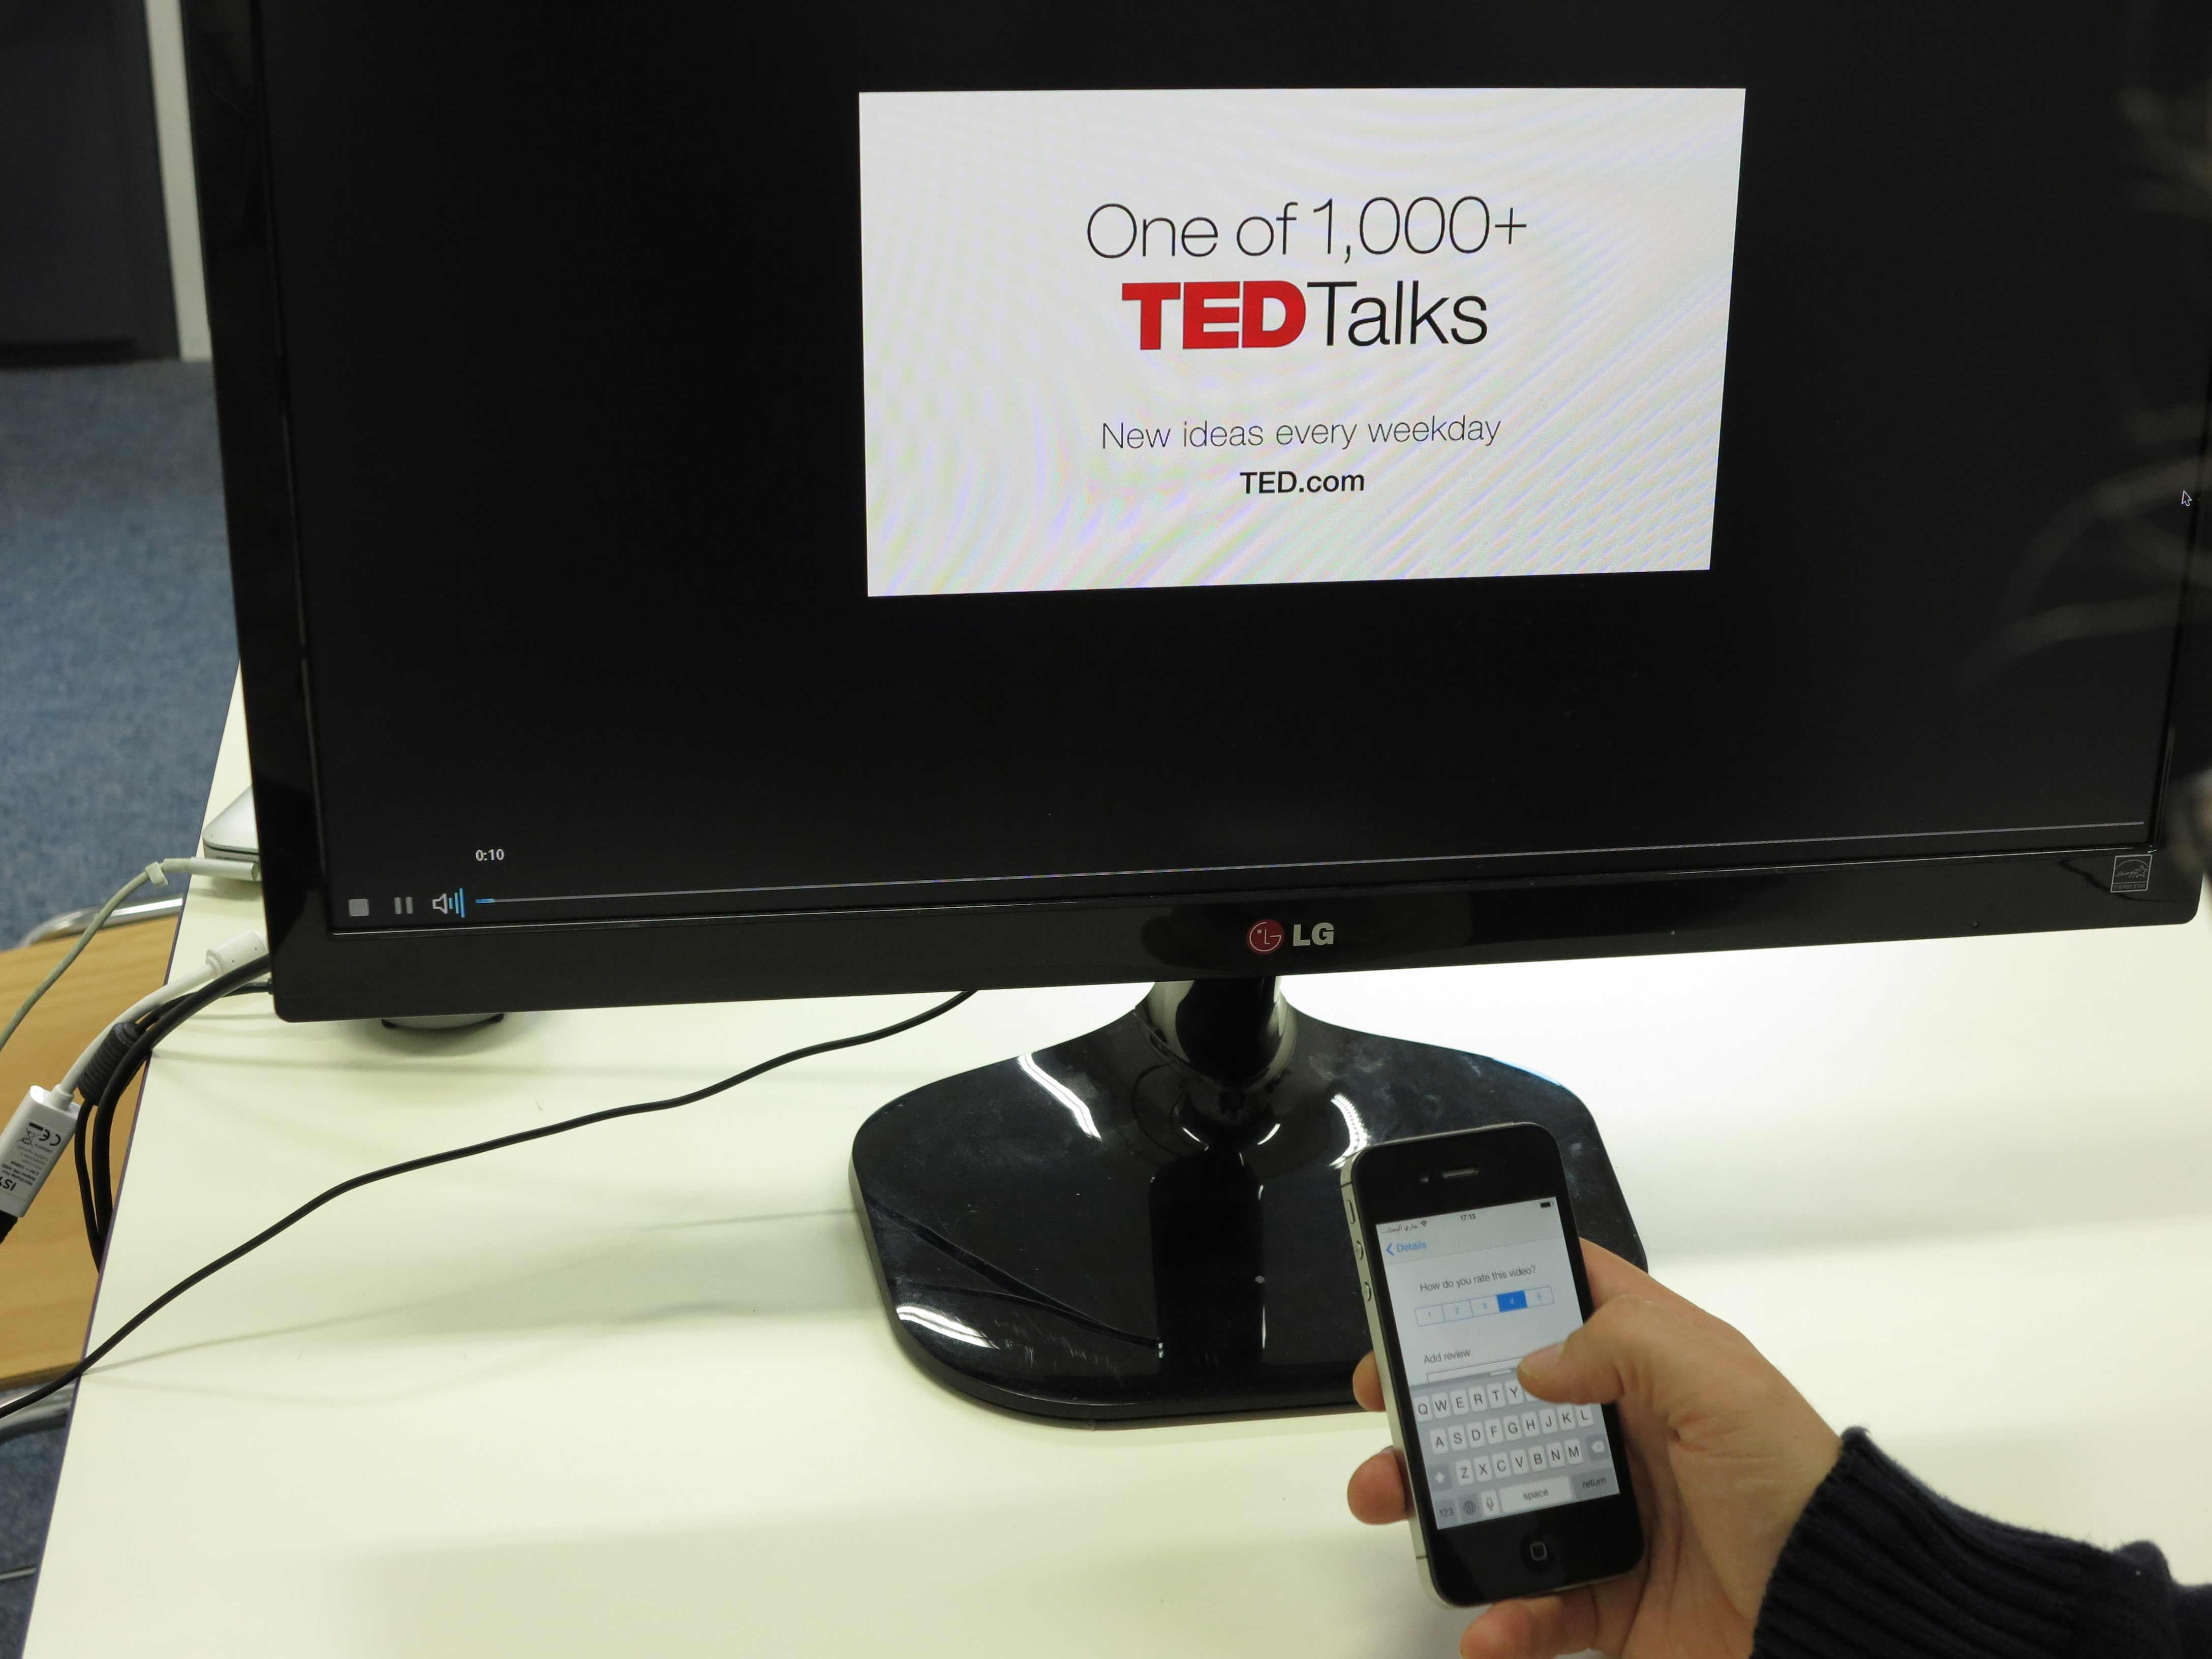
\includegraphics[width=\textwidth]{figures/IMG_6807}
        \caption{Rating and playing a video.}
        \label{fig:figure52a}
    \end{subfigure}
   
    \begin{subfigure}[b]{0.3\textwidth}
        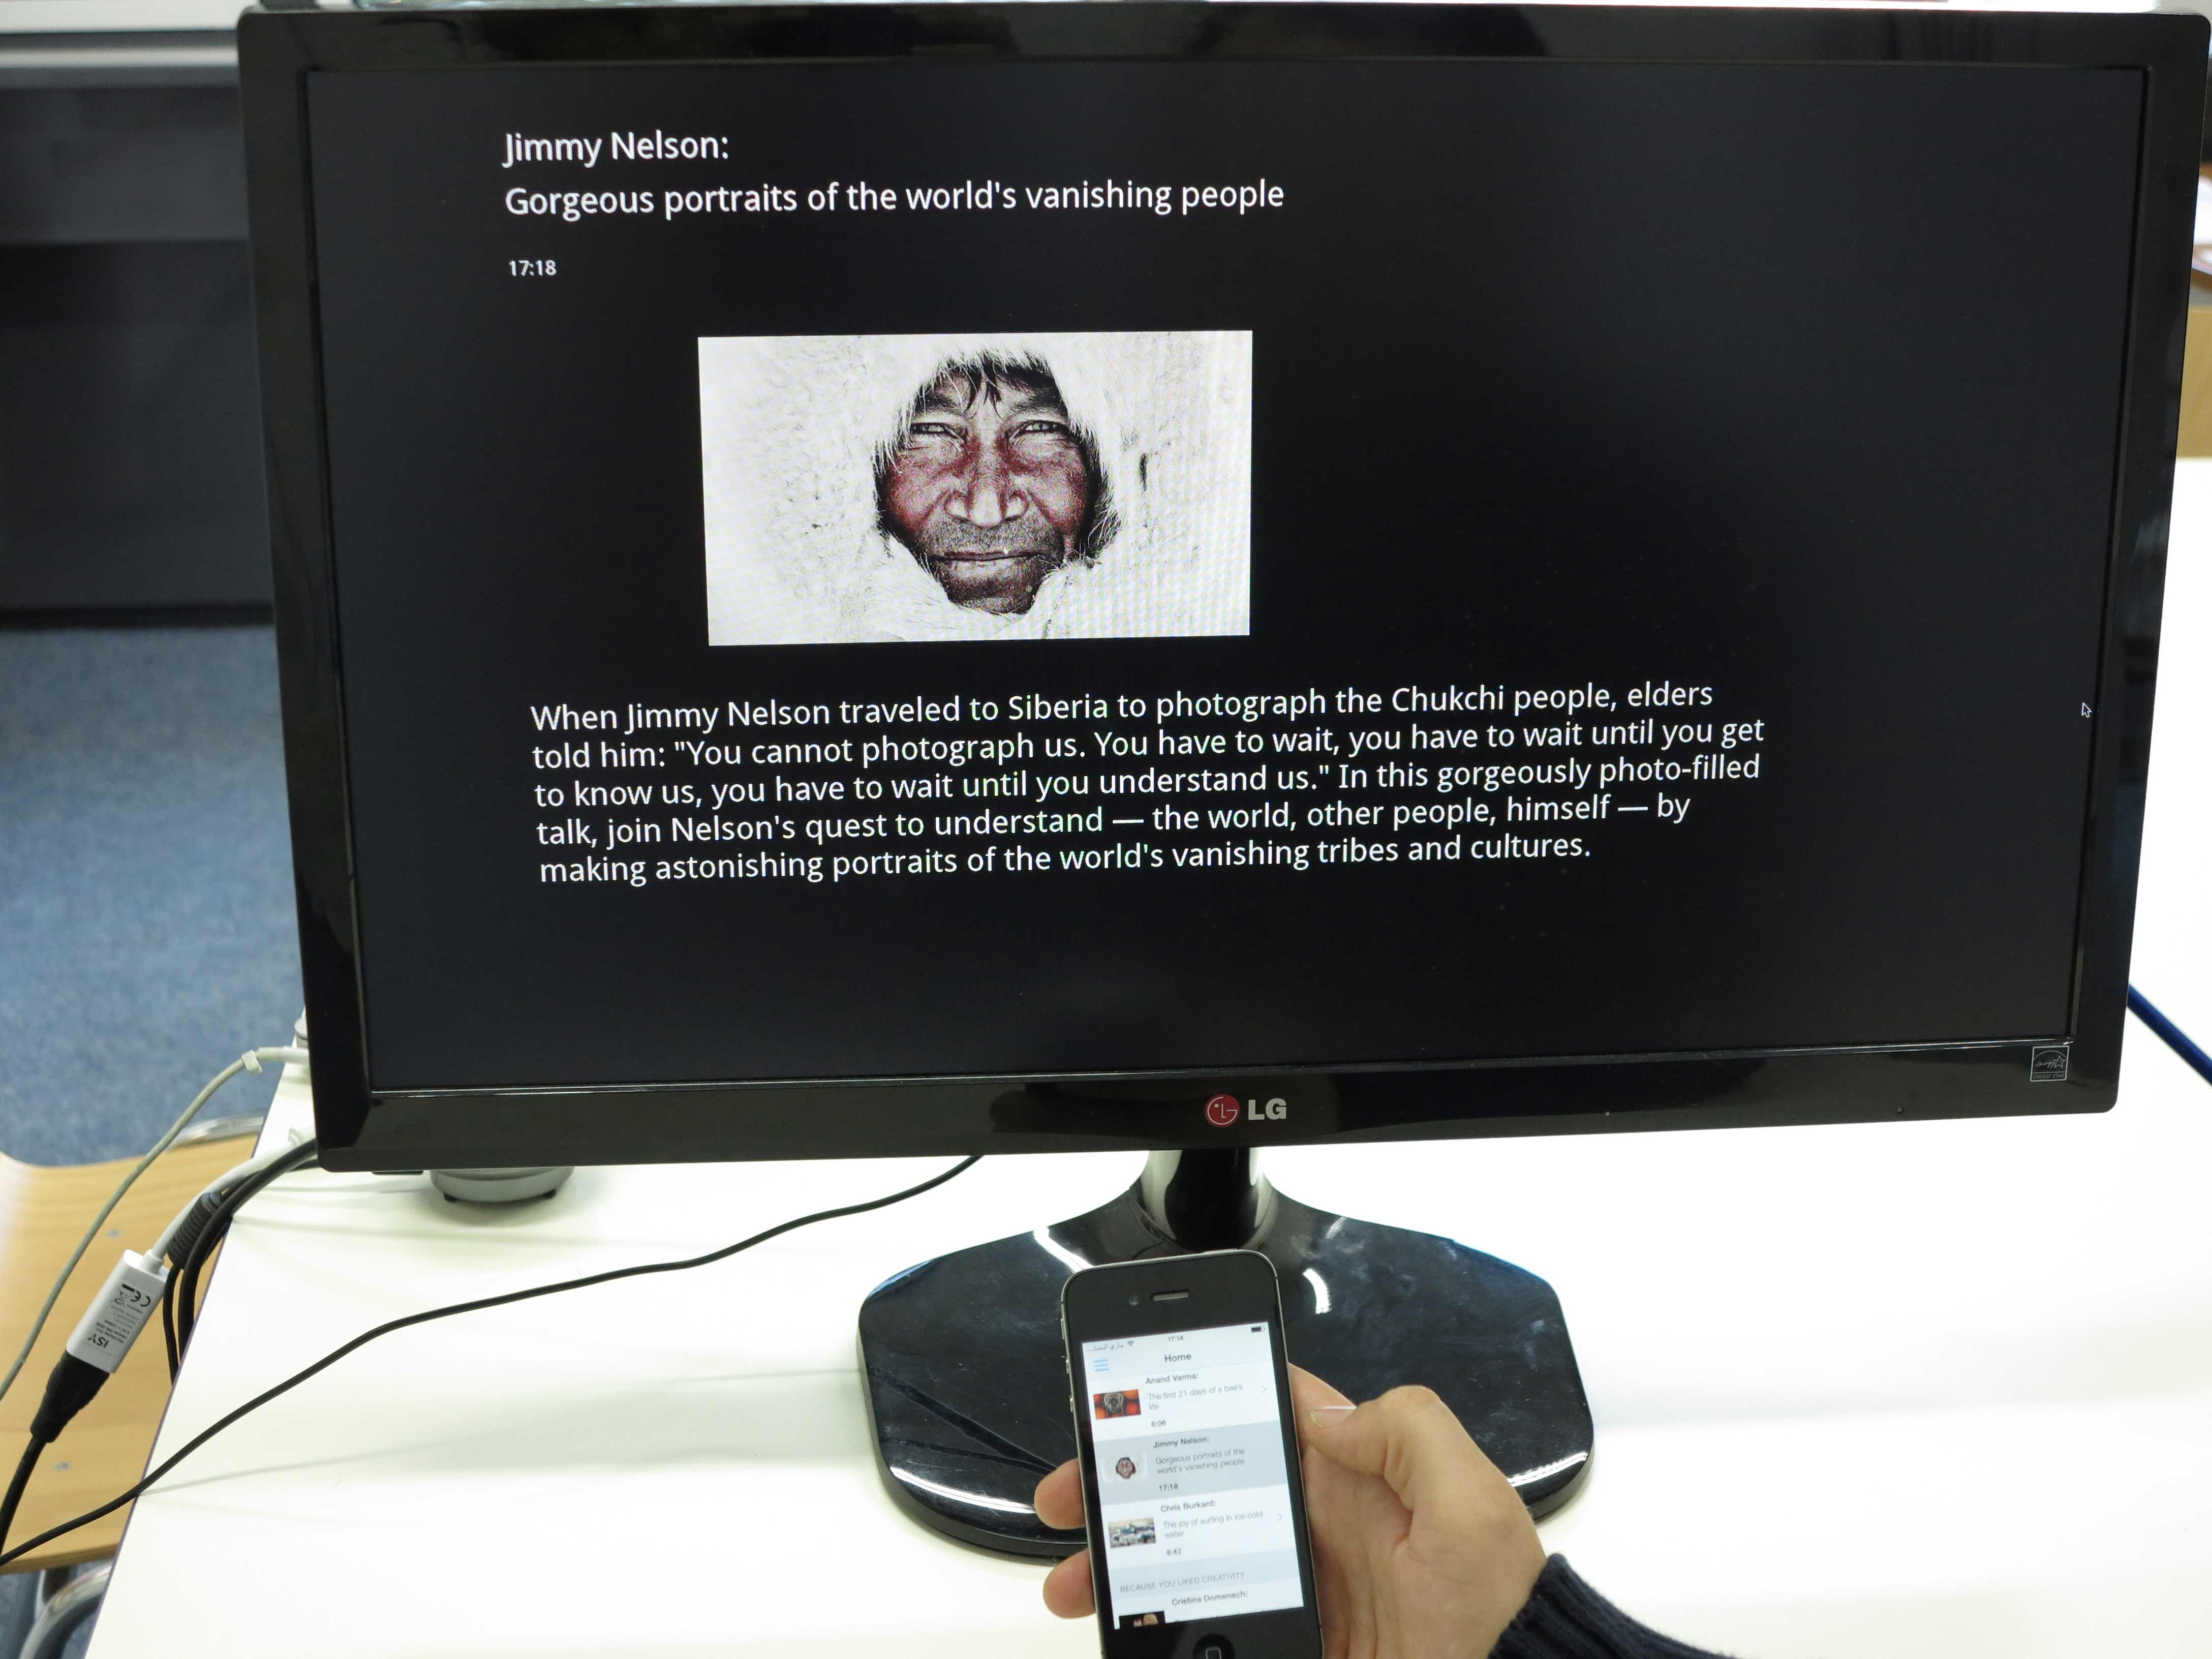
\includegraphics[width=\textwidth]{figures/IMG_6809}
        \caption{Viewing video details on DiRec}
        \label{fig:figure52b}
    \end{subfigure}
    
    \begin{subfigure}[b]{0.3\textwidth}
        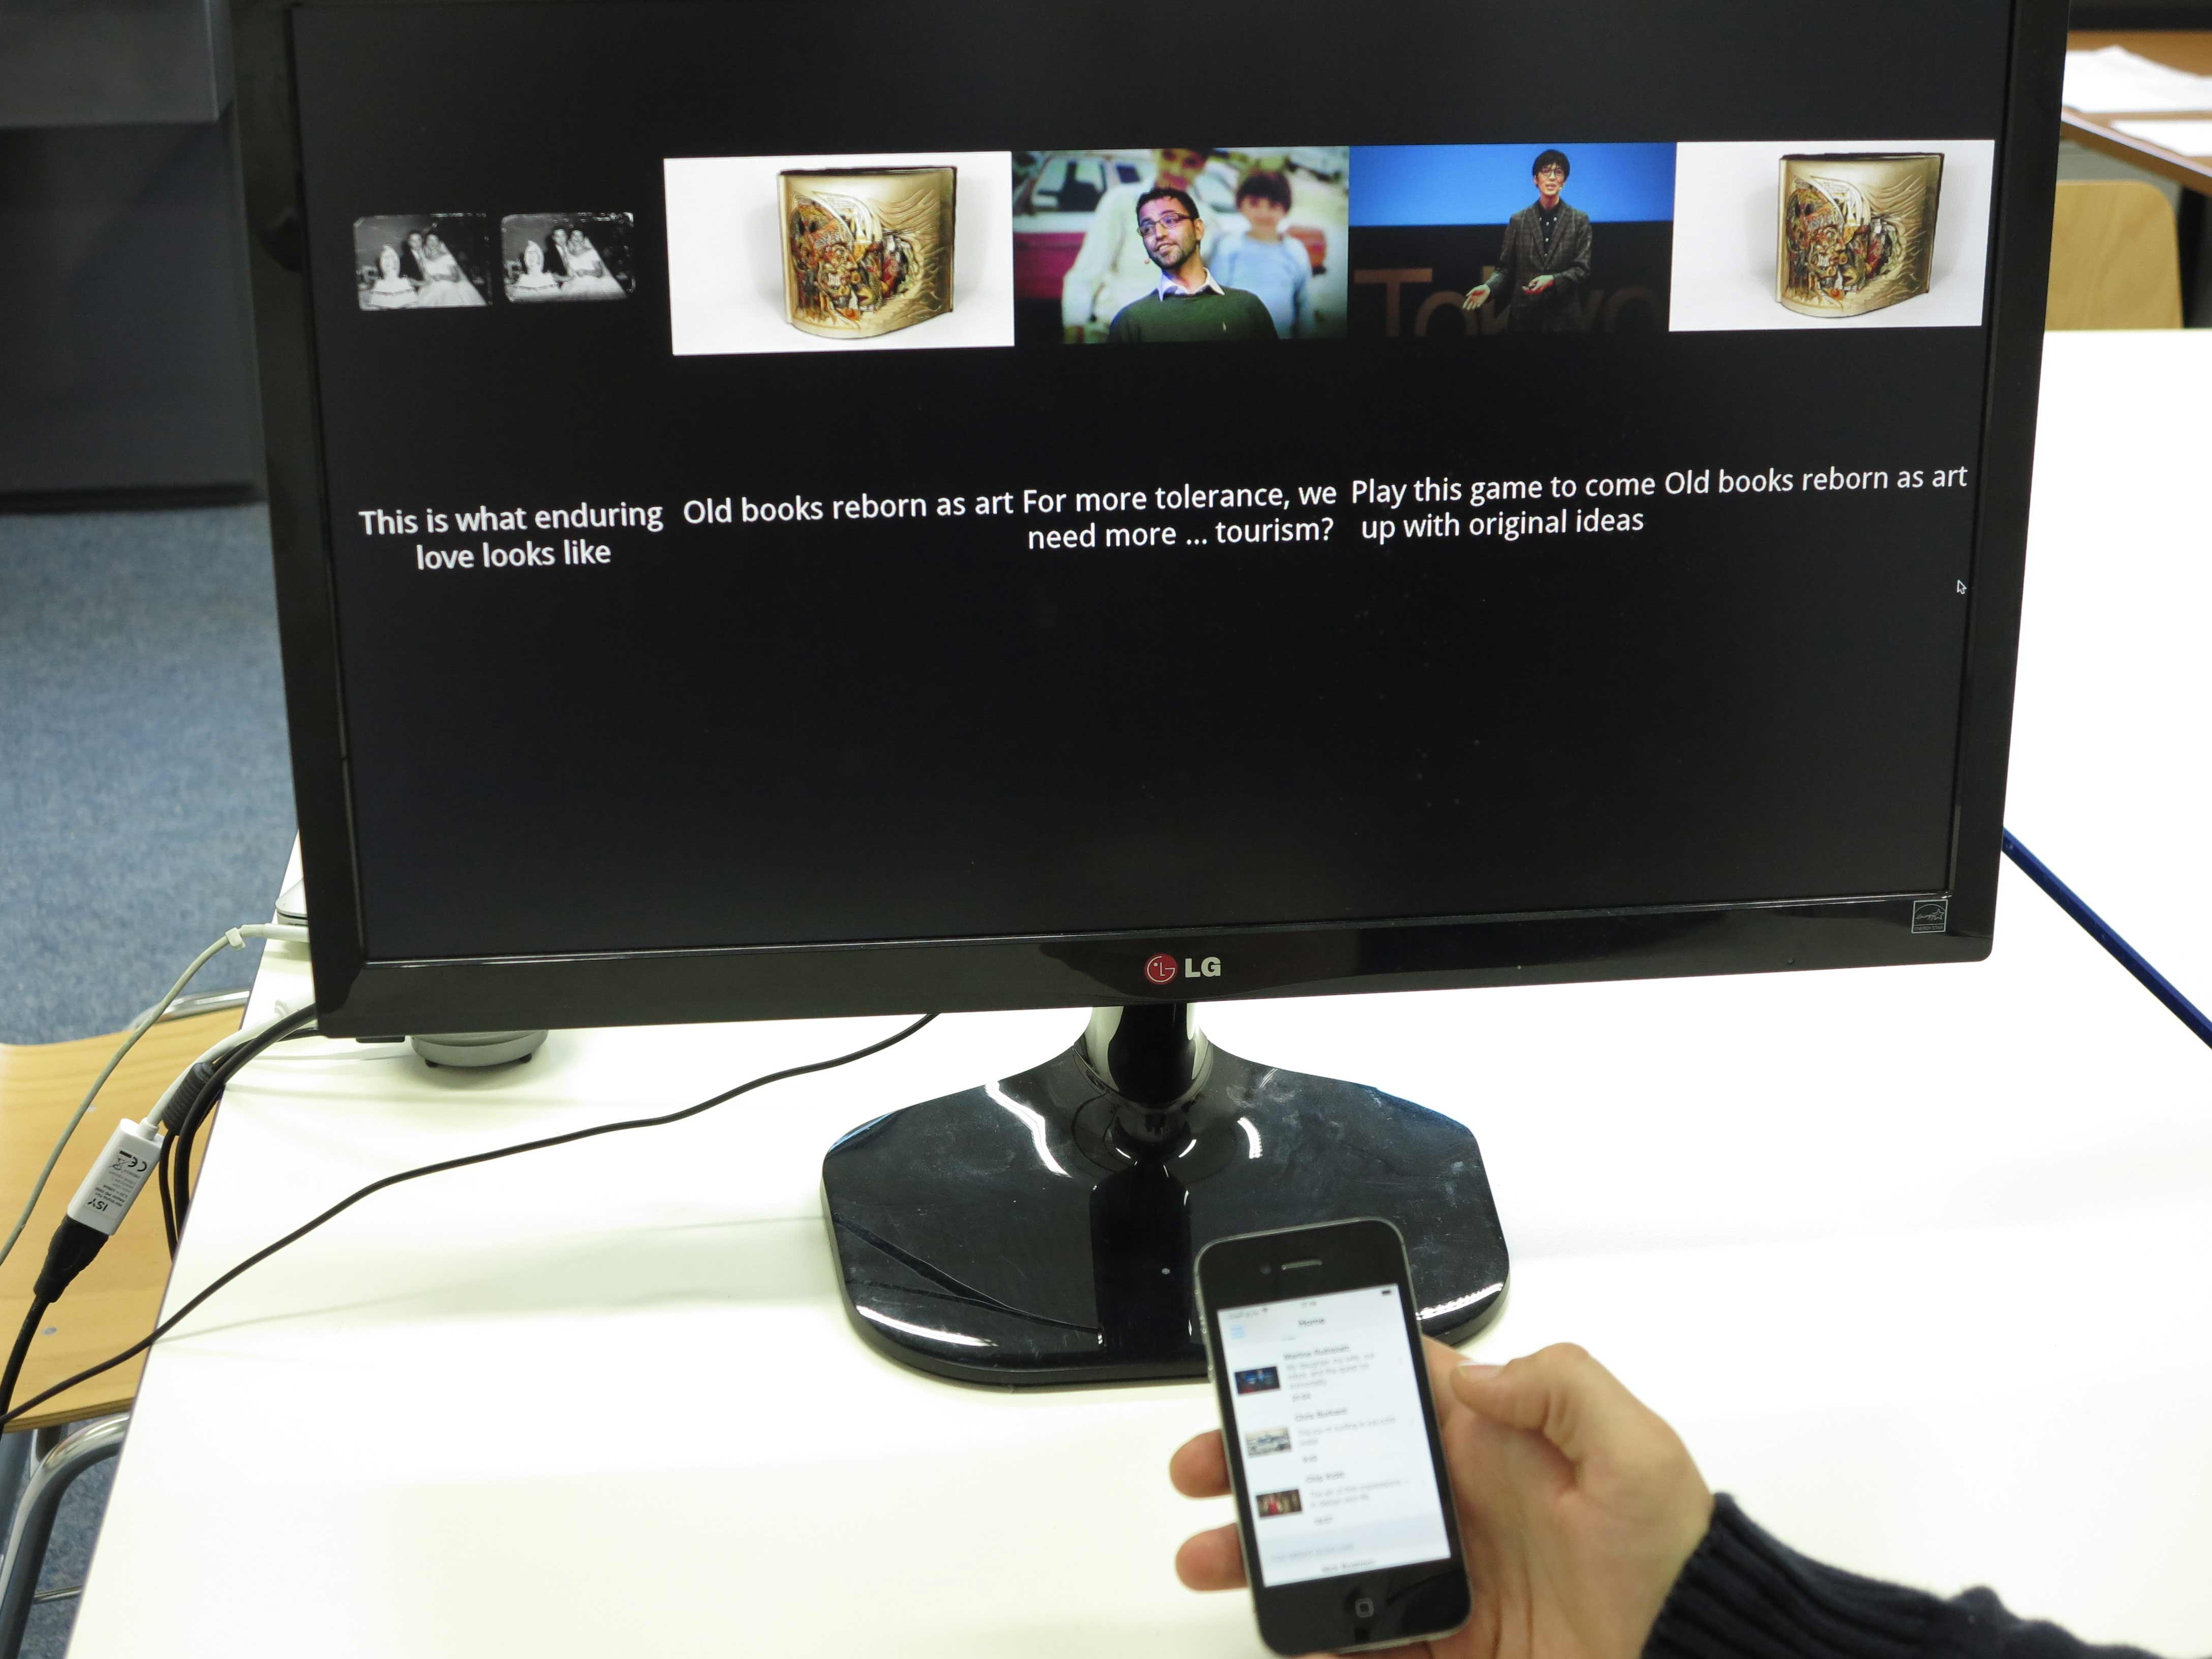
\includegraphics[width=\textwidth]{figures/IMG_6810}
        \caption{Filtering videos}
        \label{fig:figure52c}
    \end{subfigure}
   \caption{Interacting with DiRec.}\label{fig:figure52}
\end{figure}
 
\subsection{Phase 3: Post-Experiment Survey}
For eliciting participants' feedback, we use the User Experience Questionnaire
(UEQ) suggested by Laugwitz et al.
\cite{laugwitz2008construction}. This questionnaire is designed to elicit users
direct impression through rating of a set of 26 different attributes of the
apps on a scale from 1 to 7. For the study, each participant was given 2
sheets of the UEQ test and was asked to give their ratings for each app
separately, directly after she/he is done with using the apps. She/He were also
asked to not take more than 3 to 5 minutes in each evaluation, and not to analyse her
answers, as the goal is to get her overall direct impression. Appendix
show all of the 26 aspects that users were to rate. Participants were also asked
to write down their overall feedback and comment in textual form in case they
have any. Some participants preferred to give their feedback directly to us
verbally after the study was complete. We took the change to also interview some
of the participants and ask them about what she/he liked or disliked
specifically about the apps which was valuable to our analysis. Details of our
post-experiment interviews are given in the results section.

\section{Participants Demographics}
23 participants joined our study, non of which are involved directly or
indirectly in this research.
Of the 23 participants, 18 are males and 5 are females. The age range of
participants is between 23 to 31. The majority of the participants are masters
of informatics students at TU Munich, some are researchers or developers in the
same field. We assumed that all participants have no prior knowledge in
recommender systems and explained the procedure similarly to everyone regardless
of their level of expertise.

\section{Study Results}

%\begin{figure*}[t]
%\centering
%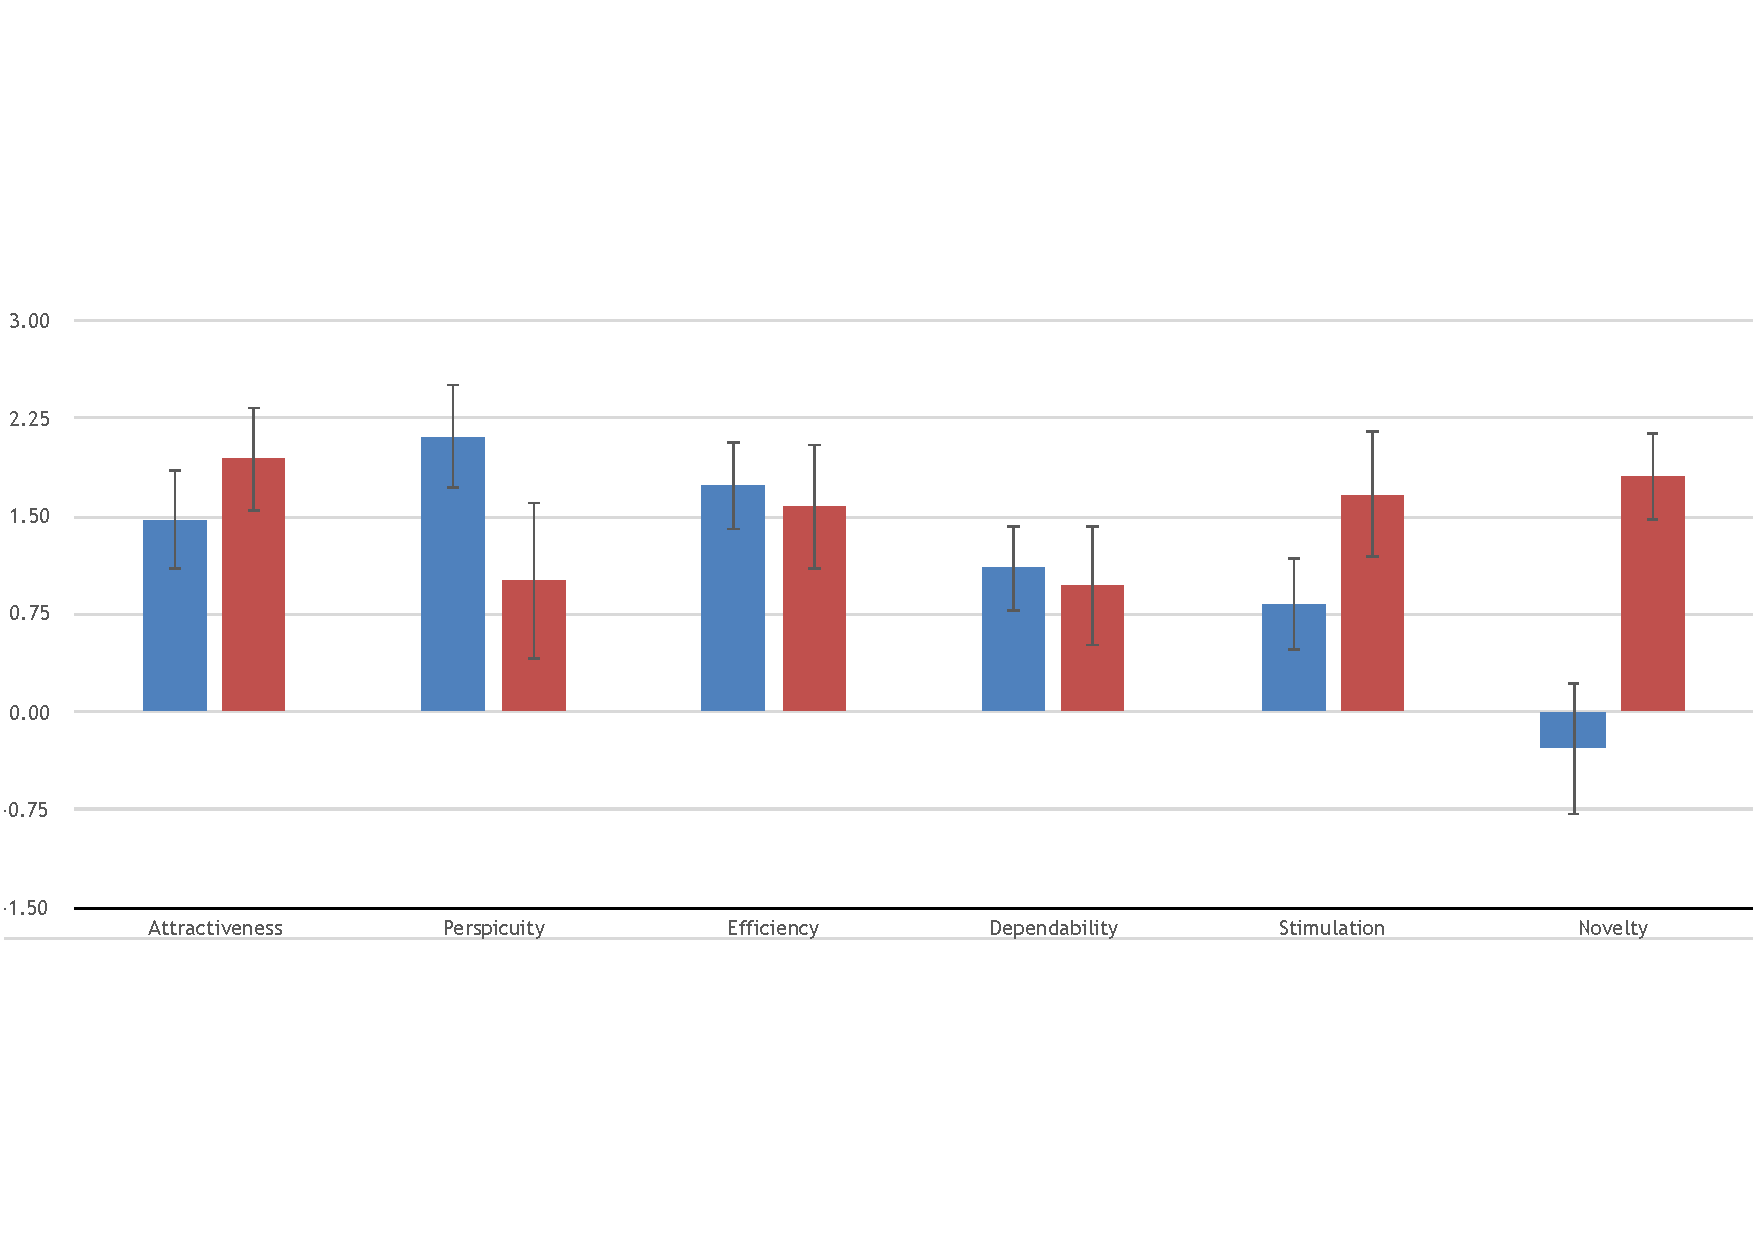
\includegraphics[width=1.0\textwidth]{figures/comparison.pdf}
%\caption{Comparison of Scale Means in MiRec and DiRec.}
%\end{figure*}


%\begin{table}[]
%\centering
%\begin{tabular}{|l|l|l|l|l|l|l|l|l|l|l|l|l|l|}
%\hline
%\multicolumn{1}{|c|}{\multirow{2}{*}{\textbf{Scale}}} &
% \multicolumn{5}{c|}{\textbf{MiRec Dataset}}                                                &                        &  & \multicolumn{6}{c|}{\textbf{DiRec Dataset}}                                                                         \\ \cline{2-14} \multicolumn{1}{|c|}{}                                & \textbf{Mean} & \textbf{STD} & \textbf{N} & \textbf{Confidence} & \multicolumn{2}{l|}{\textbf{Confidence Interval}} &  & \textbf{Mean} & \textbf{STD} & \textbf{N} & \textbf{Confidence} & \multicolumn{2}{l|}{\textbf{Confidence Interval}} \\ \hline
%\textbf{Attractiveness}                               & 1.48          & 0.89   
% & 21         & 0.38                & 1.09                     & 1.86                   &  & 1.94          & 0.88         & 19         & 0.39                & 1.55                    & 2.33                    \\ \hline \textbf{Perspicuity}                                  & 2.11          & 0.93         & 21         & 0.40                & 1.71                     & 2.51                   &  & 1.00          & 1.34         & 19         & 0.60                & 0.40                    & 1.60                    \\ \hline
%\textbf{Efficiency}                                   & 1.74          & 0.78   
% & 21         & 0.34                & 1.40                     & 2.07                   &  & 1.58          & 1.07         & 19         & 0.48                & 1.10                    & 2.06                    \\ \hline \textbf{Dependability}                                & 1.11          & 0.76         & 21         & 0.32                & 0.78                     & 1.43                   &  & 0.97          & 1.03         & 19         & 0.46                & 0.51                    & 1.44                    \\ \hline
%\textbf{Stimulation}                                  & 0.83          & 0.83   
% & 21         & 0.36                & 0.48                     & 1.19                   &  & 1.67          & 1.10         & 19         & 0.49                & 1.18                    & 2.16                    \\ \hline \textbf{Novelty}                                      & -0.27         & 1.18         & 21         & 0.50                & -0.78                    & 0.23                   &  & 1.80          & 0.74         & 19         & 0.33                & 1.47                    & 2.14                    \\ \hline
%\end{tabular}
%\caption{Comparison of Scale Means Shows the scale means and the corresponding
% 5 percent confidence intervals.}
%\label{resTable1}
%\end{table}


UEQ handook \cite{UEQHandbook}

\chapter{Conclusion And Future Work}\label{chapter:conc}



\nocite{*}  

\bibliographystyle{plain}
\bibliography{literature}

% TODO: add more chapters here
\appendix{}
\chapter{Appendix: Class Diagrams}\label{chapter:appendA}
\section{Class Diagram of MiRe/Direc}
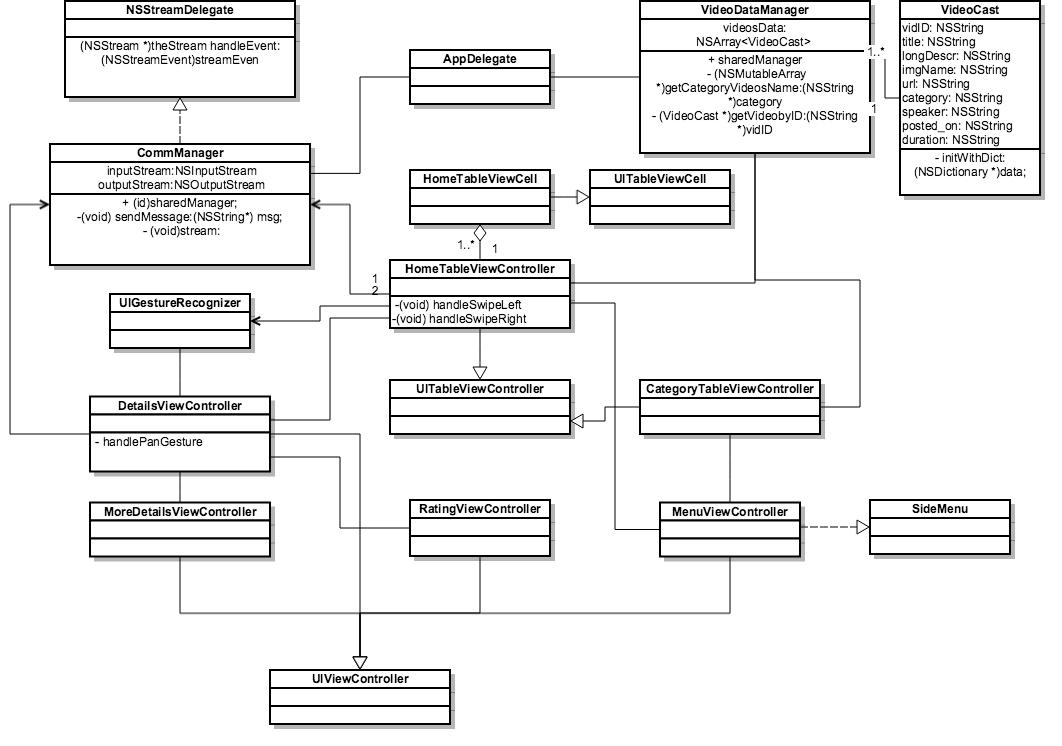
\includegraphics[width=0.9\textwidth, center, center]{figures/class_diagramSD}
\newpage
\section{Class Diagram of LD Application}
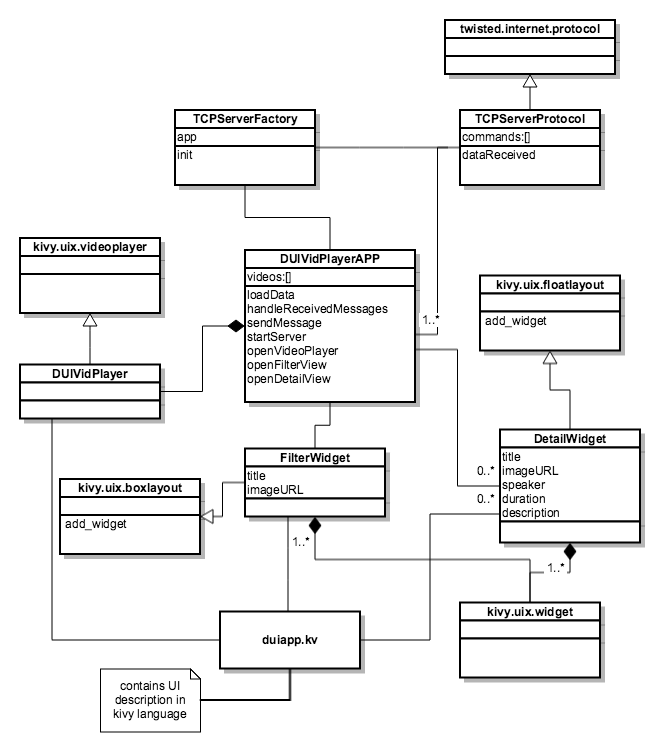
\includegraphics[width=0.9\textwidth, center, center]{figures/class_diagramLD}
 

 % TODO: remove if glossary not needed
 \glsaddall{} % add all defined terms to glossary, even if not referenced in text
 \printglossaries{}

\microtypesetup{protrusion=false}
\listoffigures{}
\listoftables{}
\microtypesetup{protrusion=true}


%\printbibliography   

  
\end{document}
